\documentclass[a4paper,titlepage]{article}
\usepackage{epsfig,amsmath,pifont,moreverb}
\usepackage{graphicx}
\usepackage{alltt}
\usepackage[colorlinks=true,
pdfpagemode=UseOutlines,
pdftitle={FASST Manual},
pdfauthor={The CRC methods group},
pdfsubject={CRC FASST},
pdfkeywords={EEG, MEG, fMRI, SPM, sleep, vizualisation, manipulation}
]{hyperref}
\pagestyle{headings}
\bibliographystyle{plain}

\hoffset=15mm
\voffset=-5mm
\oddsidemargin=0mm
\evensidemargin=0mm
\topmargin=0mm
\headheight=12pt
\headsep=10mm
\textheight=240mm
\textwidth=148mm
\marginparsep=5mm
\marginparwidth=21mm
\footskip=10mm

% Ensure paragrah are numbered and appear in TOC
%\setcounter{secnumdepth}{4}
%\setcounter{tocdepth}{4} 

% Define new characters and commands
\def\dblS{\hbox{S\hskip -4.5pt S}}
\def\dblSt{\hbox{S\hskip -6pt S}}
\def\dblSs{\hbox{S\hskip -3.5pt S}}
\def\dblSb{\hbox{S\hskip -12pt S}}

\newcommand{\bi}{\begin{itemize}}
\newcommand{\ei}{\end{itemize}}
\newcommand{\bslash}{\texttt{\symbol{92}}}
\newcommand{\matlab}{\textsc{Matlab }}
\newcommand{\Fasst}{FA\dblSb T } 	% Big shift for title page
\newcommand{\fasst}{FA\dblS T } 	% to be used in text
\newcommand{\ffasst}{FA\dblSs T } % to be used in footnotes
\newcommand{\tfasst}{FA\dblSt T } % to be used in titles


% Paragraph settings
\setlength{\parindent}{6mm}
\setlength{\parskip}{6mm plus2mm minus2mm}

%%%%%%%%%%%%%%%%%%%%%%%%%%%%
%%%%%%%%%%%%%%%%%%%%%%%%%%%%
%%%%%%%%%%%%%%%%%%%%%%%%%%%%
%%%%%%%%%%%%%%%%%%%%%%%%%%%%


\begin{document}

\newlength{\centeroffset}
\setlength{\centeroffset}{-0.5\oddsidemargin}
\addtolength{\centeroffset}{0.5\evensidemargin}

\thispagestyle{empty}
%\vspace*{3mm}
\begin{center}
	
\includegraphics[height=3cm]{images/LOGO_crc.jpg} \hfill
	
\includegraphics[height=3cm]{images/LOGO_ULg.jpg}
\end{center}
\begin{center}
	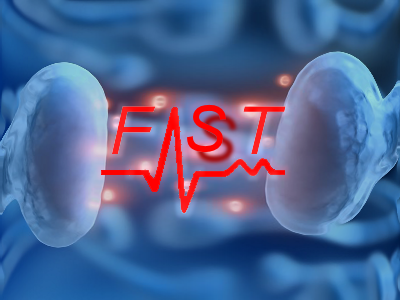
\includegraphics[width=10cm]{images/LOGO_Complex.png}
\end{center}
\vspace*{\stretch{1}}
\noindent\hspace*{\centeroffset}\makebox[0pt][l]{
	\begin{minipage}
	{\textwidth}
	\flushright
%	\textbf{\huge{fMRI artefact and Sleep Scoring Toolbox manual}}\\
	\textbf{\Huge{\Fasst manual}}
	{\noindent\rule[-1ex]{\textwidth}{5pt}\\[2.5ex]}
%	\hfill{{\huge The Cyclotron Research Centre methods group} \\}
	\hfill{{\Large \tfasst developpers at the Cyclotron Research Centre} \\}
	\vspace{8mm}
	\hfill{
	Jessica Schrouff\\
	Doroth\'ee Coppieters\\
	Remy Lehembre \\
	Yves Leclercq \\
	Pierre Maquet\\
	Quentin Noirhomme \\
	Christian Degueldre \\
	Christophe Phillips}
	\end{minipage}
}

\vspace{\stretch{2}}
\noindent\hspace*{\centeroffset}\makebox[0pt][l]{\begin{minipage}{\textwidth}
\flushright
{% \footnotesize
Cyclotron Research Centre\\
University of Li\`ege, B30\\
8 All\'ee du Six Ao\^ut\\
4000 Li\`ege, BELGIUM\\
\url{http://www.montefiore.ulg.ac.be/~phillips/FASST.html}}\\
\today
\end{minipage}}

%%%%%%%%%%%%%%%%%%%%%%%%%%%%%%%%%%%%%%%%%%%%%%%%%%%%%%%%%%%%%%%%%%%%%%%%%%%%%%%
% Table of contents
\newpage
\tableofcontents

\newpage
%%%%%%%%%%%%%%%%%%%%%%%%%%%%%%%%%%%%%%%%%%%%%%%%%%%%%%%%%%%%%%%%%%%%%%%%%%%%%%%
\section{Introduction}
\label{sec:Introduction}
%%%%%%%%%%%%%%%%%%%%%%%%%%%%%%%%%%%%%%%%%%%%%%%%%%%%%%%%%%%%%%%%%%%%%%%%%%%%%%%

``\fasst\hspace{-4pt}'' stands for ``fMRI Artefact rejection and Sleep Scoring Toolbox''. This M/EEG toolbox is developed by researchers from the Cyclotron Research Centre, University of Li\`ege, Belgium, with the financial support of the Fonds de la Recherche Scientifique-FNRS, the Queen Elizabeth's funding, and the University of Li\`ege.
On Dr. Pierre Maquet's impulse we started writing these tools to analyze our sleep EEG-fMRI data and tackle four crucial issues:
\begin{description}
	\item[Continuous M/EEG.]Long multi-channel recording of M/EEG data can be enormous. These data are cumbersome to handle as it usually involves displaying, exploring, comparing, chunking, appending data~sets, etc.
    \item[EEG-fMRI.]When recording EEG and fMRI data simultaneously, the EEG signal acquired contains, on top of the usual neural and ocular activity, artefacts induced by the gradient switching and high static field of an MR scanner. The rejection of theses artafacts is not easy especially when dealing with brain spontaneous activity.
    \item[Scoring M/EEG.]Reviewing and scoring continuous M/EEG recodings, such as is common with sleep recordings, is a tedious task as the scorer has to manually browse through the entire data set and give a ``score'' to each time-window displayed.
    \item[Waves detection.] Continuous and triggerless recordings of M/EEG data show specific wave patterns, characteristic of the subject's state (e.g., sleep spindles or slow waves). Their auomatic detection is thus important to assess those states.
\end{description}
Currently the toolbox can efficiently deal with these issues, as described in section \ref{sec:functions}. Eventhough the toolbox was originally divised for EEG data, it also handles MEG and LFP data without any problem, if in the right format (see section \ref{sec:datachan}). 
\fasst is in effect an add-on toolbox for SPM8\cite{SPM8,Litvak2011} and relies on SPM8 data format and functions to perform some operations.

Troubles usually come from the data format and channel setup but see section \ref{sec:datachan} for \fasst requirements and solutions. The ``eye-balling'' and manipulation of continuous multi-channel recordings is eased by a series of tools (see section \ref{sec:GeneralTools}).
Specifically, for EEG-fMRI acquisitions (see section \ref{sec:eeg_fmri}), \fasst can operate directly on the raw data acquired with a ``BrainAmp MR'' system (Brain Products GmbH, Gilching, Germany) and includes the well-known AAS method\cite{Allen2000} for the ``gradient artefact'' rejection, as well as the recently published ``constrained ICA'' method\cite{Leclercq2009} for the rejection of the ``pulse artefact''. Other ``classic'' methods for the ``pulse artefact'' rejection are also available. And an easy GUI is available for the manual scoring of sleep EEG by different users (see section~\ref{sec:Sleeptools}). Some statistics and sleep specific features can then be automatically extracted.

\fasst is available for free, under the GNU-GPL and, obviously, it comes without any warranty: you should use it at your own risk. This is an ongoing research project and we plan to add new features and functionalities, according to our own needs and the feedback from users. If you are happy with the results obtained with \fasst and publish them, please use the following references:
\bi
\item for the toolbox in general and the sleep specific tools\cite{CRCtb,Leclercq2011}
\begin{alltt}
J. Schrouff, D. Coppieters, R. Lehembre, Y. Leclercq, P. Maquet,
Q. Noirhomme, C. Degueldre, E. Balteau, and C. Phillips,
fMRI Artefact rejection and Sleep Scoring Toolbox (FASST).
Cyclotron Research Centre, University of Li\`ege, Belgium, 2009.
http://www.montefiore.ulg.ac.be/~phillips/FASST.html
\end{alltt}
and
\begin{verbatim}
Y. Leclercq, J. Schrouff, Q. Noirhomme, P. Maquet, C. Phillips,
``fMRI Artefact rejection and Sleep Scoring Toolbox'',
Computational Intelligence and Neuroscience, 2011.
http://www.hindawi.com/journals/cin/2011/598206/
\end{verbatim}
\item for the constrained ICA ``Pulse artefact'' rejection method\cite{Leclercq2009} in particular
\begin{verbatim}
Y. Leclercq, E. Balteau, T. Dang-Vu, M. Schabus, A. Luxen, P. Maquet, and
C. Phillips.
``Rejection of pulse related artefact (PRA) from continuous electroencepha-
lographic (EEG) time series recorded during functional magnetic resonance
imaging (fMRI) using constraint independent component analysis (cICA)'',
NeuroImage, 44(3):679-691, 2009.
\end{verbatim}
\ei
Note that \fasst includes a few routines from 3 other freely available toolboxes:
\bi
\item EEGLAB\cite{Delorme2004,Delorme2011}, mainly for a few functions used by the constrained ICA ``pulse artefact'' rejection, available from \url{http://sccn.ucsd.edu/eeglab/};
\item the FMRIB plug-in for EEGLAB\cite{FMRIBplugin}, for the ECG peak detection and classic PCA/Gaussian mean ``pulse artefact'' rejection, available from \url{http://users.fmrib.ox.ac.uk/~rami/fmribplugin/}; 
\item the ``Mutual Information computation'' package\cite{Peng2005}, for some the selection of correction matrices during cICA ``pulse artefact'' rejection, available from \url{http://penglab.janelia.org/proj/mRMR/}.
\ei
We thank their authors for letting us use their work.

We would also be thankful to hear from you if you find bugs in the code.
Feel also free to submit add-ons to this toolbox but please note that support will not be provided for ``home-made'' changes of the distributed code.

%%%%%%%%%%%%%%%%%%%%%%%%%%%%%%%%%%%%%%%%%%%%%%%%%%%%%%%%%%%%%%%%%%%%%%%%%%%%%%%
\section{Installing \& launching the toolbox}
\label{sec:Installation}
%%%%%%%%%%%%%%%%%%%%%%%%%%%%%%%%%%%%%%%%%%%%%%%%%%%%%%%%%%%%%%%%%%%%%%%%%%%%%%%

%CORRECTIONS to include for next release:
%- no need to change the subsref.m function in filearray!
%- note about recompiling the MInfo function using the makeosmes.m function


In order to work properly, \fasst needs to have those 2 softwares installed:
\bi
\item a recent version of \matlab, we used version~7.5~(R2007b) to develop \fasst\hspace{-4pt}. Any later \matlab version should work, {\it in theory}.
\item the latest version of the ``Statistical Parametric Mapping Software'', i.e. SPM8 \cite{SPM8,Litvak2011}. You can download it from: \url{http://www.fil.ion.ucl.ac.uk/spm/software/}. Install it in a suitable directory, for example {\tt C:\bslash SPM8\bslash }, and make sure that this directory is on the \matlab path\footnote{No need to include the subdirectories!}.
\ei

{\bf NOTE:} Originally \fasst relied on routines from \matlab ``Signal Processing Toolbox''  for some filtering functions. In this version we have tried to lift this requirement. If you do not have the toolbox, filtering and time-frequency operations are executed by freely available equivalents\footnote{see in the subdirectory {\tt \bslash FASST\bslash SPTfunctions}.} distributed under the GNU General Public License .

\subsection{Installation}
%--------------------------------------

After registering and downloading the zipped file containing \fasst\hspace{-4pt}, the installation proceeds as follow:
\begin{enumerate}\addtolength{\itemsep}{-1\baselineskip}
\item	Uncompress the zipped file in your favourite directory, for example {\tt C:\bslash FASST\bslash };\\
%\item	Copy and overwrite the content of the subfolder ``{\tt To copy in spm\_@filearray}'' into the subfolder \linebreak ``{\tt @filearray}'' in the SPM8 folder\footnote{The {\tt subsref.m} function distributed with this toolbox works faster (at least on our win-XP and win-Vista computers) for large data files ($>$200Mb) and is necessary for the toolbox to work in some cases (e.g. extremely arge data set >2Gb).};\\
\item	Launch \matlab ;\\
\item	Go to the ``{\tt File}'' menu $\rightarrow$ ``{\tt Set path}'';\\
\item	Click on the ``{\tt Add folder}'' button and select the \fasst folder, i.e. {\tt C:\bslash FASST\bslash } if you followed the example;\\
\item	Click on save.
\end{enumerate}

A few routines from the ``Mutual Information computation'' package\cite{Peng2005} are written in C++ ({\tt .cpp} files) and should thus be compiled for your specific operating system. We are providing these compiled routines for the usual OS's such as: Windows XP (32 bits), Windows 7 (64 bits), Mac OS 10, Linux (32 bits). If your OS is not listed (or routines do not work properly), you can compile the routines with the {\tt makeosmex.m} script available in the {\tt MInfo} subdirectory.

\subsection{Launching and batching}
%--------------------------------------

Once installed, there are three ways to call up \fasst functionalities: %\hspace{-4pt}
\bi
\item to launch the toolbox GUI, just type {\tt crc\_main} or {\tt fasst} at the \matlab prompt and the main GUI figure will pop up, see Fig. \ref{fig:crc_main}. From there on simply click on the tool you want to use;
\item some functions of \fasst have been integrated into SPM8 {\tt matlabbatch} batching system \cite{matlabbatch}, the batching GUI is launched by typing {\tt crc\_batch} at the \matlab prompt\footnote{check SPM8's manual for more information about matlabbatch};
\item most tools can also be called individually by calling them directly from the \matlab prompt, or for scripting in a {\tt .m} file.
\ei
\begin{figure}[ht]
	\centering
		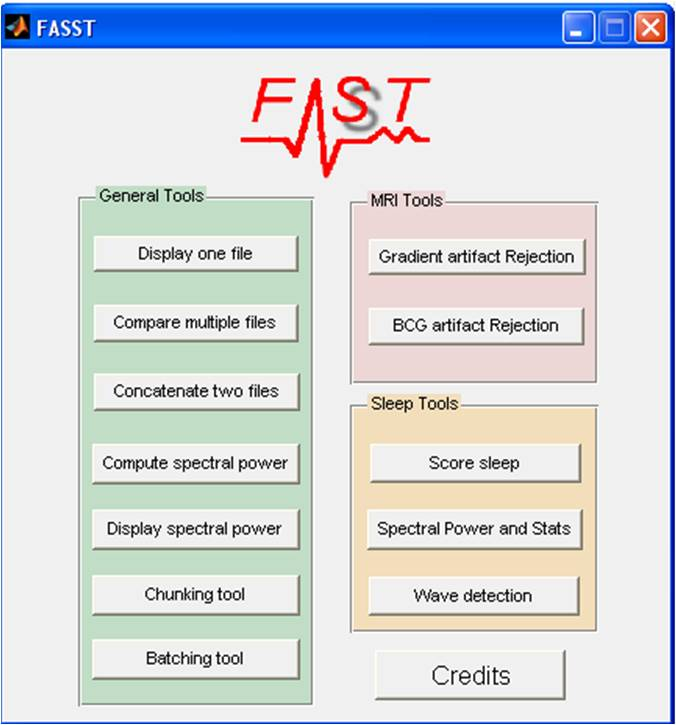
\includegraphics[width=8cm]{images/FIG1_crc_main.JPG}
	\caption{Main GUI window. The 3 families of tools (General, EEG-fMRI, and sleep) are clearly seperated.
	\label{fig:crc_main}}
\end{figure}	

%%%%%%%%%%%%%%%%%%%%%%%%%%%%%%%%%%%%%%%%%%%%%%%%%%%%%%%%%%%%%%%%%%%%%%%%%%%%%%%
\section{Data format \& channels setup}
\label{sec:datachan}
%%%%%%%%%%%%%%%%%%%%%%%%%%%%%%%%%%%%%%%%%%%%%%%%%%%%%%%%%%%%%%%%%%%%%%%%%%%%%%%

Data format is always an issue in EEG and MEG since each company enjoys his own specific (and usually proprietary) format. So we decided to use the \matlab based and open SPM8 {\tt meeg} data format. Therefore \fasst internally works with SPM8 {\tt meeg} data format:
\bi
\item a {\tt .mat} ``header'' file, which contains all the information about the data (channel names and types, sampling rate, stimuli, data format, etc.) as well as room for user-specific data; and
\item a {\tt .dat} binary file\footnote{it's only a binary finale, so any extension could be used actually, and that's what \ffasst does sometimes.}, which  stores the recorded data themselves as a raw list of numbers\footnote{By default SPM8 saves the data as {\tt FLOAT} but other format, e.g. {\tt INT16} can be used.}.
\ei
The resulting data files are also stored in that format.  Informations, like the sleep score encoded by users, are simply added to the header data structure and do not interfere with SPM8 machinery. Advanced users are advised to have a look at SPM8's manual for a description of the SPM8 M/EEG tools and data format.

 Data can thus be imported in two ways, either via SPM8 ``convert'' function or directly via \fasst\hspace{-4pt}: 
\bi
\item SPM8 relies on the ``FieldTrip'' (FT) toolbox \cite{Fieldtrip,Oostenveld2011} to read in and convert a very large number of EEG/MEG data formats (pretty much any format that exists). SPM8 generally reads in the header and creates the {\tt .mat} ``header'' file, then goes through the data file and creates the {\tt .dat} binary file. The 2 files created have the same name as the original data but prepended with ``{\tt spm8\_}''.
\item \fasst directly handles far fewer data format than SPM8-FT. So far only Brain Products  (Brain Products GmbH, Gilching, Germany), raw-exported EGI (Electrical Geodesics Inc., Eugene, OR, USA), {\tt EDF} \cite{Kemp1992,Kemp2003,EDF} and {\tt BCI2000} (\url{http://www.bci2000.org/}) data formats are directly supported. Those types of data can be directly selected via \fasst GUI and are converted `on the fly'. There is therefore no ``import'' button in \fasst\hspace{-4pt}.
\ei

\fasst import can be faster for the supported format but SPM8/FT approach is probably the safest for any other format, as both SPM8/FT are constantly improved. Nevertheless depending on the way raw original data are stored on disk, SPM8/FT can more than double the size of your data on disk\footnote{Sometimes raw EEG data are saved in {\tt INT16} format, i.e. 2 bytes per sample, but SPM8/FT converts them to {\tt FLOAT}, i.e. 4 bytes per sample.}.
In both cases, before any `advanced processing', i.e. anything more than just having a look at the signal, it is advisable to check the channel informations (type, scale, units, name, 2D location, etc.) using SPM8 {\tt meeg} reviewing function.

% This still presents 2 advantages. First, those types of data can be directly selected via the \fasst GUI and they'll be converted ``on the fly''. Second, Brain Products EEG data (e.g. acquired during fMRI with a BrainAmp) are imported without generating a second data file (see section~\ref{sec:dataBP}).

% Therefore, if \fasst defaults are properly setup for your data (channel names, location, type, etc.), if your EEG data set has been acquired with a BrainProducts amplifier, especially for simultaneous EEG-fMRI recording (see section \ref{sec:dataBP}), or is in another format supported by \fasst (see section \ref{sec:dataother}), you can directly select it in the GUI and the conversation will take place automatically. There is therefore no ``import'' button in \fasst\hspace{-4pt}.
% For any other data format, you should first convert your data set using SPM8 functionalities\footnote{In this case the raw binary file is copied and the 2 files created ({\tt *.mat} and {\tt *.dat}) are prepended with ``{\tt spm8\_}''.}, before using it in \fasst\hspace{-4pt}. Note that SPM8 offers facilities to easily edit channel and data information via a GUI, check the SPM8 manual for more informations.

\subsection{Data format conversion with \tfasst}
%--------------------------------------
\label{sec:dataconvert}

When converting data with \fasst, there is a bit more information that can be retrieved than with SPM8/FT. If the recording time of the data, i.e. clock time of the beginning of the recording, is available, then that information is extracted and saved in the {\tt meeg} object. This information can be useful for
\bi
\item single file display. For example with night long recording, it's easier to be able to look at the 'real world' recording time instead of the time elapsed since the beginning of the recording
\item multiple file display. The display of multiple data files (raw vs. chunked and filtered for example) is then synchronized on the 'real worl' recording time.
\item data handling. When chunking or appending data set(s), the 'real world' recording time is accounted for.
\ei

\subsubsection{Brain Products data format conversion}
%--------------------------------------
\label{sec:dataBP}

\fasst can {\it directly} read and import raw data from the Brain Products (Brain Products GmbH, Gilching, Germany) EEG amplifiers: BrainAmp, QuickAmp and V-Amp\footnote{V-Amp special edition have crypted headers (with a {\tt .ahdr} extension), you need to export the data to ``binary data format'' in order to obtain the {\tt *.vhdr} and {\tt *.dat} files.}. EEG recorded for several hours at the row (like in a sleep study) or during fMRI acquisition usually generates massive data files (up to several Gb for fMRI-sleep recordings!) due to recording duration and the high sampling rate (typically 5kHz for EEG-fMRI). Being able to read and process these raw data without a lengthy exportation/importation procedure or the need to make copies of this huge data file, was thus particularly important for us. Since we own BrainAmp MR amplifiers for EEG-fMRI recording (as many other laboratories do), we focused on their data format.

The raw data from BP amps consist in three files, for example {\tt fname.eeg}, {\tt fname.vhdr}, {\tt fname.vmrk}, which are respectively the binary data file, the header file and the marker file.
The header and marker files are simple text files. These two are directly read in by \fasst and translated into SPM8 data structure\footnote{This includes the triggers recorded along side the EEG.}, which is then directly linked to the binary data file. Thus be aware that the binary data file containing the data is {\bf NOT} copied at this ``importation'' stage! The following processing step(s), for example the ``gradient artefact removal'' (see section \ref{sec:gar}), will thus access the {\it original} binary data file. Even though the original binary data should never be overwritten by \fasst\hspace{-4pt}, it is still advisable to keep a safe copy of your orginal ``raw data'' in a safe place.
%Other (raw) data formats should be imported via SPM8 importation routine. In this case the raw binary file is copied and the 2 files created ({\tt *.mat} and {\tt *.dat}) are prepended with ``{\tt SPM8\_}''.

\subsubsection{Other data format conversion}
%--------------------------------------
\label{sec:dataother}

Raw continuous {\tt EDF}, EGI and {\tt BCI2000} data formats are now supported by \fasst but some restrictions apply: %\hspace{-4pt}
\bi
\item {\tt EDF} data set sometimes have channels with different sampling rates. Channels with lower sampling rates, usually physiological measures (breathing, CO2, etc.) are simply upsampled to the highest sampling rate, usually the EEG channel, in order to have the same sampling rate for all channels. Note also that .edf data are assumed to be in a {\tt INT16} format, which is usually the case but not necessarily so.
\item EGI data should be continuous ``raw exported'' data. For the moment, the data file is read in and re-written on disk after removing the channels associated with the triggers/inputs\footnote{It should be possible though to avoid reading-and-writing the big data file on disk and directly access the original raw data. Maybe in a future update...}. These trigger/inputs are turned into events in the SPM8 {\tt meeg} object.
\item {\tt BCI2000} data importation is only a {\it beta} version!
\ei
As stated above, other (raw) EEG/MEG data formats should be imported via SPM8 importation routine. In this case the raw binary file is copied and the 2 files created ({\tt *.mat} and {\tt *.dat}) are prepended with ``{\tt spm8\_}''.

\subsection{Channel definition}
%--------------------------------------
\label{sec:chandef}
Channel definition (name, type, sacele, unit, 2D-location, etc.) is in line with that of SPM8. Therefore it is strongly advisable to use SPM8's review function to set up the channel informations properly and, possibly, apply a montage to re-reference all or some channels. 
Still within the toolbox we use an enhanced ``channel setup'' file ({\tt CRC\_electrodes.mat})  specific to EEG recordings, and introduce an extra bit of information ``{\tt crc\_types}'' for the channels. This allows the on-the-fly display of bipolar montage along EEG channels and the use of different channel scalings, e.g. for EEG and ECG channels, for the display. Most common channel names are already available within the toolbox. If you used a lab-specific setup (and most everyone does...) or weird channel names, you should then add those channels to {\tt CRC\_electrodes.mat}.
For more information on how to adjust the channel definitions to your specific channel setup, please read and edit the function {\tt crc\_electrodes.m}. A new {\tt CRC\_electrodes.mat} is then generated by executing {\tt crc\_electrodes.m}. % Another possibility is to manually edit the channel informations via SPM8's GUI, though SPM8 does not know about the ``{\tt crc\_types}'' field.

%%%%%%%%%%%%%%%%%%%%%%%%%%%%%%%%%%%%%%%%%%%%%%%%%%%%%%%%%%%%%%%%%%%%%%%%%%%%%%%
\section{Main functions of the toolbox}
\label{sec:functions}
%%%%%%%%%%%%%%%%%%%%%%%%%%%%%%%%%%%%%%%%%%%%%%%%%%%%%%%%%%%%%%%%%%%%%%%%%%%%%%%

The following tools and features are available in the current version of \fasst\hspace{-4pt}:
\bi\addtolength{\itemsep}{-1\baselineskip}
\item	General tools \\
\bi\addtolength{\itemsep}{-1\baselineskip}
\item Displaying one M/EEG data file\\
\item Comparing multiple M/EEG data files\\
\item Appending M/EEG data files into a single data file\\
\item Chunking a time window from an M/EEG data file\\
\item Computing the spectrogram of one M/EEG data file\\
\item Displaying the spectrogram or power spectrum of an M/EEG data file\\
\ei
\item EEG-fMRI artefact rejection tools\\
\bi\addtolength{\itemsep}{-1\baselineskip}
\item Gradient artefact rejection: AAS method\\
\item Pulse artefact rejection: AAS, `Gaussian mean' and cICA methods\\
\ei
\item Sleep specific tools\\
\bi\addtolength{\itemsep}{-1\baselineskip}
\item Manual sleep scoring\\
\item Spectral power calculations and statistics\\
\ei
\item Automatic wave detection tools\\
\bi\addtolength{\itemsep}{-1\baselineskip}
\item Slow waves (SW)\\
\item sleep spindles (SP, {\it beta version}) 
\ei
\ei

\subsection{General tools}
%=========================
\label{sec:GeneralTools}

These are tools to display, review, compare, process, manipulate and handle (long) multichannel continuous data files.

\subsubsection{Displaying one M/EEG data file}
%--------------------------------------
\label{sec:dis_main}
This tool is designed to display multiple channels of one continuous M/EEG recording and browse throughout the data. The display routine includes built-in ``on-screen'' filtering and %\linebreak
 re-referencing function. There is therefore no need to perform these pre-processing steps before visualizing the data. In fact you can use these options to see what would be the effect of filtering or re-referencing on your data.

When you launch the display routine, the selection channel interface appears first. At this point you have to choose the list of channels you want to look at. To select a channel, you just have to click on its name in the left hand column (Fig.~\ref{fig:TB_disselchan}-A). The name of this channel will disappear from the left column and appear in the right column (Fig.~\ref{fig:TB_disselchan}-B). The channels recognized by the toolbox, i.e. with 2D-localisation information, will appear in the lower right white box (Fig.~\ref{fig:TB_disselchan}-C) according to their position on the scalp. Some buttons allow you to automatically select a set of electrodes (Fig.\ref{fig:TB_disselchan}-D). When you have selected all the channels of interest, click on the `PLOT' button to launch the display interface (Fig.~\ref{fig:TB_disselchan}-E). The `SCORE' button (Fig.~\ref{fig:TB_disselchan}-F) leads to the same display but with the scoring tools and menu enabled, see section~\ref{sec:Sleepscoring}.
\begin{figure}[ht]
	\centering
		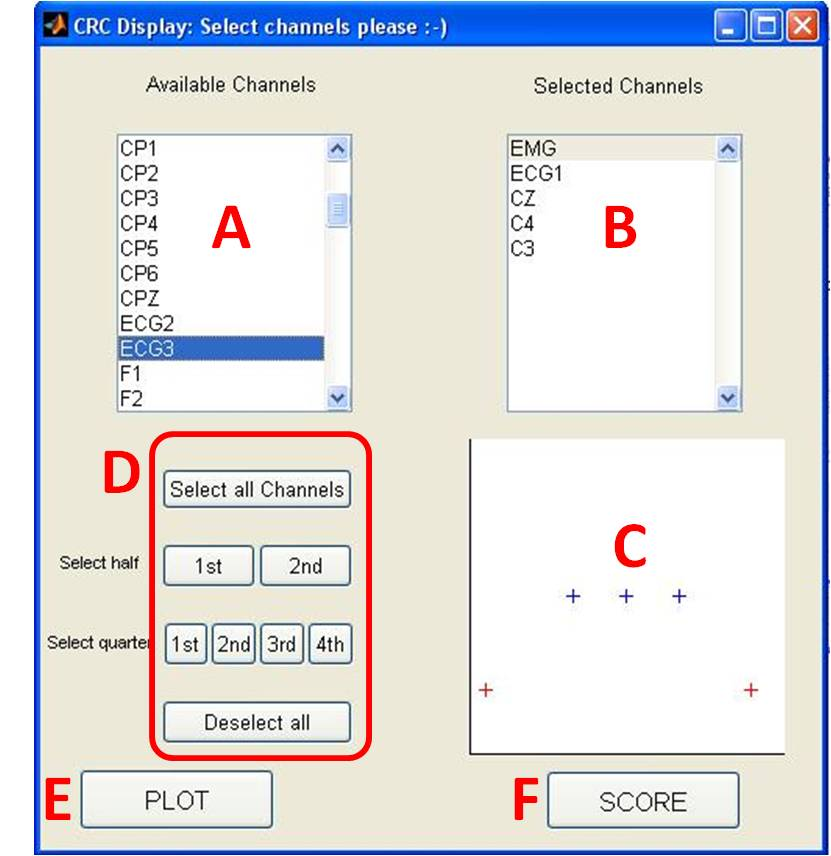
\includegraphics[width=8cm]{images/FIG2_dis_selchan.jpg}
	\caption{Channel selection GUI: A. channel list, B. selected channels, C. selected channels 2D-location, D. pre-specified automatic channel selection, E. plot selected channels, F. plot selected channels and score the signal.
	\label{fig:TB_disselchan}}
\end{figure}	

A display window appears with the channel display in the main central box (Fig.~\ref{fig:TB_dismain}-A). The scaling, time window settings, number of channels displayed, re-referencing and filtering option are on the right part of the window (Fig.~\ref{fig:TB_dismain}-B). There are two scrolling bars: one to quickly browse throughout the data over time, below the channel display (Fig.~\ref{fig:TB_dismain}-C), and another one to browse through sub-sets of selected channels, on the right of the channel display (Fig.~\ref{fig:TB_dismain}-D).
\begin{figure}[ht]
	\centering
		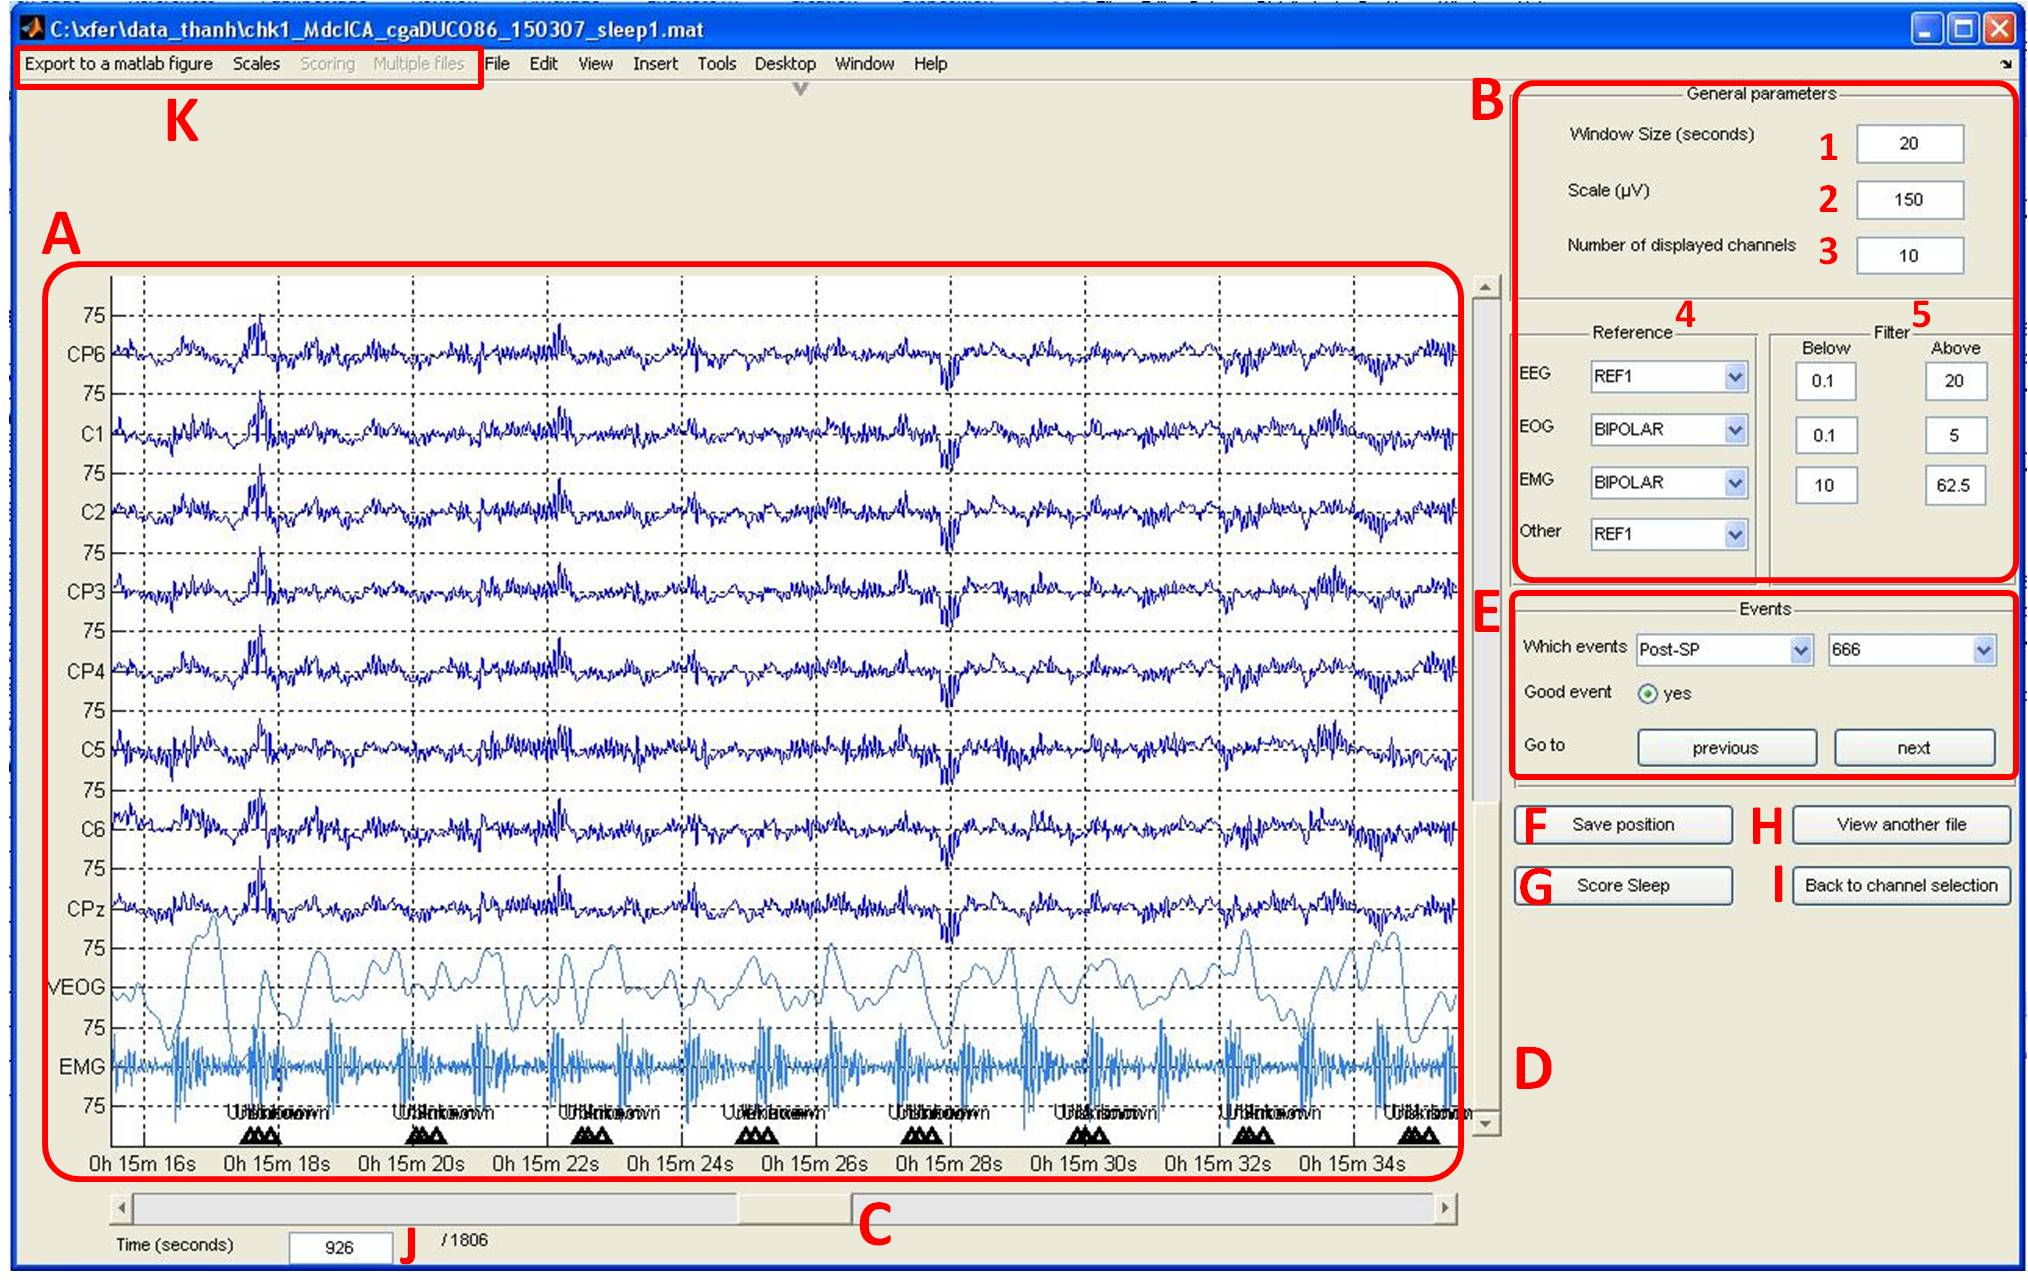
\includegraphics[width=15cm,height=10cm]{images/FIG3_crc_dis.jpg}
	\caption{Channels display window: A.~main display, B.~display options (see text for details), C.~time scrolling bar, D. go to sleep scoring, E.~view another file, F.~back to channel selection, G.~time in seconds at the beginning of display, H.~export display to a \matlab figure.
	\label{fig:TB_dismain}}
\end{figure}

In the main display window (Fig.~\ref{fig:TB_dismain}-A), standard unipolar channels are displayed in dark blue, electrocardiographic (EKG or ECG) in red and the others in lighter blue. The scaling of the various channels will depend on their type, as defined in the SPM8 {\tt meeg} object. If this information is not available (poor importation or the data have not been ``properly'' prepared) then \fasst uses the {\tt crc\_types} variable of the channel setup file {\tt crc\_channels.mat} to find the channels that are automatically rescaled and the bipolar montages\footnote{In this case, it will not be possible to scale correctly EEG and MEG channels simultaneously!}.

The `Window Size' (Fig.~\ref{fig:TB_dismain}-B1) fixes the length of the window displayed (in seconds).  The `Scale' setting fixes the relative distance in $\mu V$ between two channels in the main window (Fig.~\ref{fig:TB_dismain}-B2). The number between two channel labels stands either for minus half the scale for the above channel and for plus the half scale for the lower channel. 
This scale indicates a signal of reference in the order of 150$\mu V$. Channels with other units will be rescaled according to their type (see the `Scales' pull-down menu (Fig.~\ref{fig:TB_dismain}-K), while the `Scale' value (Fig.~\ref{fig:TB_dismain}-B2) will act on the signal of all channels at once.
For example if you fixed the scale at 150 $\mu V$, 75~will appear between label channels and the scale of each EEG channel goes from  -75 $\mu V$ to~+75~$\mu V$. The `Number of displayed channels' (Fig.~\ref{fig:TB_dismain}-B3) fixes the number of channels per screen (to see the other channles, scroll up or down). 

The `Reference' panel (Fig.~\ref{fig:TB_dismain}-B4) allows you to re-reference the data to a chosen reference. For the EEG channels, this reference may be any other channels (even if you did not select it in the channel selection interface), the mean of all the EEG channels or the mean of the two mastoids (called M1 and M2). For the EOG and EMG channels you have an additional `Bipolar' choice for the reference. Pairs of EOG (and EMG) channels are usually designed to work as a bipolar montage, let's say that EMG1 and EMG2 are specified to be referenced to each other. If you only display EMG1 and choose the bipolar reference, then EMG1 will be displayed referenced to EMG2. Note that this re-referencing relies on the channel names and is performed only `on-display' (the original data stored on disk are left untouched).

The `Filter' panel (Fig.~\ref{fig:TB_dismain}-B5) allows you to bandpass filter the various types of channels differently. The cut-off frequencies are indicated in the boxes next to the channel type. Like the re-referencing, this filtering is performed only `on-display' and the original data stored on disk are left untouched. 

The `Save Position' button  (Fig.~\ref{fig:TB_dismain}-F) allows you to store the time your time cursor is currently at and, when opening the same file later, your time cursor will be replaced at that position. Useful when reviewing waves or when scoring very long files.
The `Score Sleep' button (Fig.~\ref{fig:TB_dismain}-G) allows you to launch the scoring utility to score the file you are currently displaying. The `View another file' button (Fig.~\ref{fig:TB_dismain}-H) allows you to select another file to display and, eventually, the `Back to channel selection' button (Fig.~\ref{fig:TB_dismain}-I) lets you go back to the channel selection interface.

The box below the time-slider shows the current time~(Fig.~\ref{fig:TB_dismain}-J), in the middle of the display window, expressed in seconds, from the beginning of the recording; the other number is the overall length of the recording also expressed in seconds. You can type in a value to jump directly to any moment of interest in the recording.

Events comprised in the data set are displayed as small triangles on the display. The `events' panel  (Fig.~\ref{fig:TB_dismain}-E) allows to scroll through these events, by first choosing which events type and value to display (respectively the left and right pull-down menus) and then using the `previous� and `next' buttons to move to the nearest previous and next event. The events types and values are those saved in the {\tt events} field of the data.

For the case where waves (e.g. slow waves or sleep spindles) were automatically detected (see section \ref{sec:WaveDetect}), some specific codes are used:
\bi
\item for spindles, the event type would be `spindles', `Post-SP' or `Ant-SP', with code values of 777, 666 or 555 respectively. 'spindles' are marked when no wavelet analysis is used during detection, otherwise they are differentiated into posterior or anterior spindles (`Post-SP' and `Ant-SP' respectively). 
\item For slow waves, the event types are either `SW' (codes starting with 3) or `delta' (code starting with 4). 
\ei
The `events number' option from the right pull-down menu lets you display the values of the selected events instead of their type\footnote{For example, this is useful when you're dealing with EEG-fMRI data and scanner triggers are numbered, then you display scan numbers along the EEG signal}. Using the `good event' radio button, individual events can be marked as good (by default, value 1) or bad (0). Events marked as `bad' appear in red on the display. The good/bad values of all events are saved in a new `goodevents' field specific to \fasst in the {\tt meeg} object. For spindles and slow waves particularly, the values are also saved in the `spindles' and `SW' fields, created when detecting the waves. Note that any change in the event numbering or any new wave detection will overwrite this information\footnote{Therefore, we would advise to perform this event marking after all analyses, especially wave detections, are done.}. Finally, when displaying a slow wave, a `map of delay' radio-button will be visible. When checked, a propagation map of the current SW (based on the SW delay) is displayed. The 2D channel location either comes from default CRC channels positions (`auto') or the positions of your channels (`file', then select your file). 

A series of pull-down menus are available in the upper part of the main display window (Fig.~\ref{fig:TB_dismain}-K). There is a button allowing you to export the current plot to a new \matlab figure. This may be handy if you plan to save the displayed signal as an image file. Next to this menu, a `Scales' menu is also available, letting you enter directly the scale of certain types of channels: defined as $10^x$, with x representing the factor of your signal of interest compared to your original data. For example, if you have EEG channels recorded in Volts (V), the scale should be $10^{-6}$, since the signal of interest is in $\mu V$.

Finally you can compute the power spectrum on one channel of the signal you are currently seeing. To do so, right click next to the signal of interest in the main window, select `Compute power spectrum on this channel' and a new \matlab figure will appear (Fig.~\ref{fig:TB_dismainpwr}) showing you the power spectrum of the signal on the window displayed and on the designated channel.
\begin{figure}[ht]
	\centering
		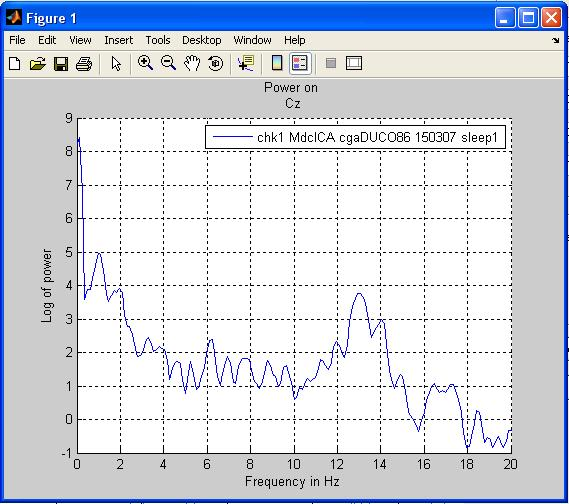
\includegraphics[width=8cm,height=4cm]{images/FIG4_dis_pwr.jpg}
	\caption{Power spectrum of the signal displayed from the designated channel.
	\label{fig:TB_dismainpwr}}
\end{figure}


\subsubsection{Comparing multiples M/EEG data files}
%--------------------------------------------
This tool is designed to display the same channel from multiple M/EEG files. It can obviously be used to compare the results of different artefact correction methods applied on the same data set or to visually check the effect of a series of ``filtering'' steps applied on a data set (Fig.~\ref{fig:TB_discmp}). This routine is the same as the main display, except that some functionalities are hidden and others added. Instead of displaying multiple channels from one file, it will display one common channel from multiple files. The `Multiple files' pulldown menu is enabled, which allows you to display the filenames, change the selected channel to display, and exit the display. 

When the tool is launched, you simply select multiple EEG files. The program will automatically compare the channels recorded in each file. The channels common to all files will be available for display. Only one channel can be displayed at one time. The displayed channel can be modified via the `Multiple files' menu.

The routine also checks the beginning time of each recording (if available) and aligns the different EEG time series in consequence. If the beginning time was not imported from the raw data (or was manually deleted at some point), it is assumed that all files begin at the same time: their first time bin. Otherwise the ``true'' beginning time of each file is used: if for some time window, some signal is missing from one data set (e.g., you chunked out the 1st few seconds of a data set before filtering it) then that data channel is left empty.

\begin{figure}[ht]
	\centering
		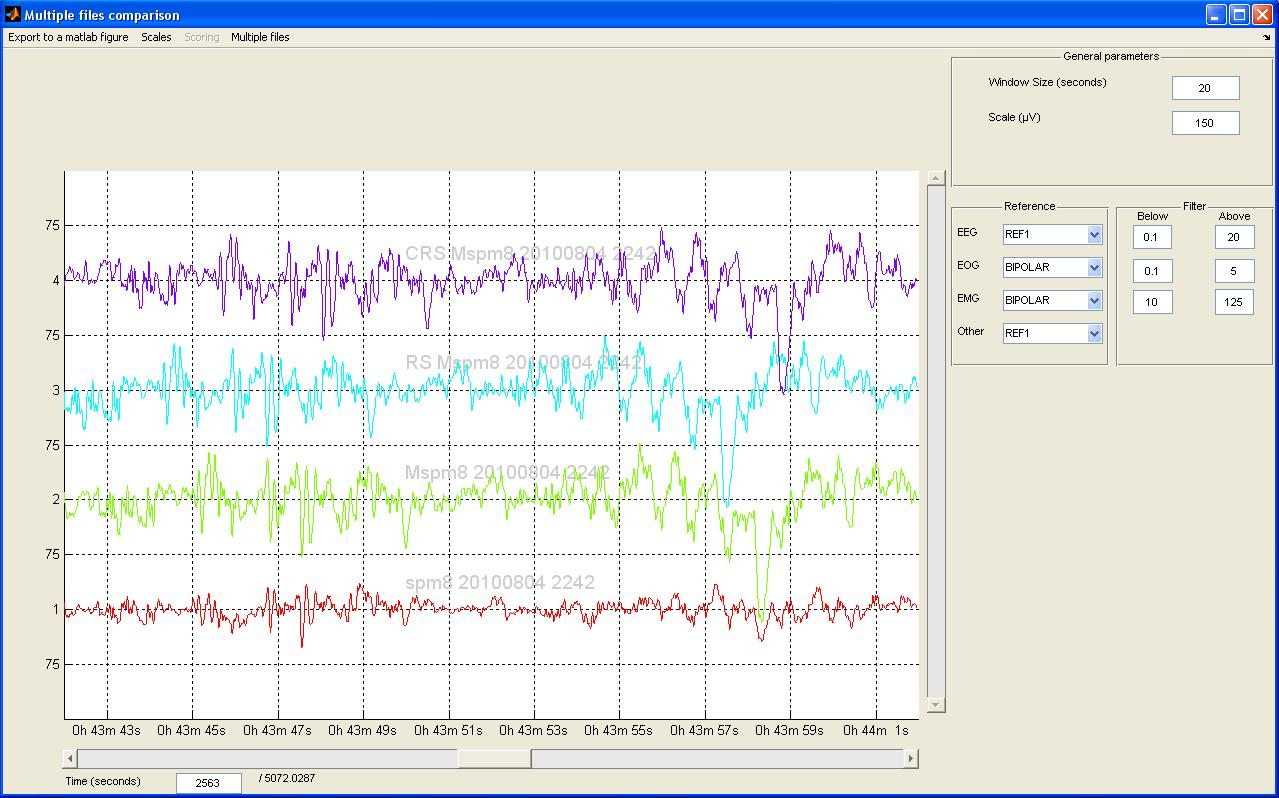
\includegraphics[width=15cm,height=9cm]{images/FIG5_dis_cmp.jpg}
	\caption{Multiple files comparison GUI, with some features from the main display GUI and others specific to this data comparison GUI.
	\label{fig:TB_discmp}}
\end{figure}

Contrary to the colour scheme of the main display tool, here the different files are simply displayed in different colours to differentiate them. 
If you right-click on the displayed signal, you may display the power spectrum of the displayed channel for one or all of the signals currently displayed .

\subsubsection{Appending M/EEG data files}
%-----------------------------------
\label{sec:appending}
Sometimes during long recording session, the operator may need to stop the recording to fix some problem, or recording may be accidentally interrupted. So for one ``recording session'', the user ends up with two (or sometimes more...) EEG files. This tool is designed to append those separate EEG files into a single one.

The routine works with two files at a time. So when you have more than two files, you should append the first two files which creates a new file that you append with the third, and so on:
\bi
\item If the 'real world' recording time of each file is available, the routine first checks the 'real world' begining time of each file, and automatically determines the file order. Then it fills the gap between the end of the first data set and the beginning of the second by zero's, and eventually appends the second the file.
\item If no 'real worl' time information is available in the file (after using the SPM8/FT conversion for example), the routine will ask if you want to operate a `blind concatenation'. In this case, the routine supposes that there is no missing samples between the consecutive file and that you entered the files in the correct order.
\ei
In both cases, the resulting file has the same name as the first file selected prefixed with {\tt cc\_}. 

\subsubsection{Chunking a time window from an M/EEG data file}
%----------------------------
\label{sec:chunking}
This tool allows the user to cut out an episode out of a large EEG file and save it as a different EEG file. This can be useful if one wants to study specific activity such as sleep stages, epileptic discharge,... The beginning and end of the new file can be defined by a marker or by time (Fig.~\ref{fig:TB_chunk}).

\begin{figure}[ht]
	\centering
		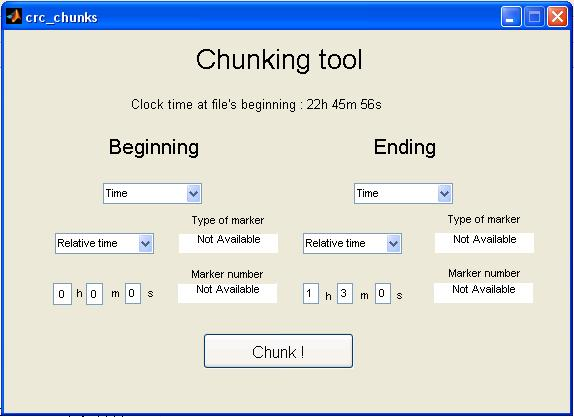
\includegraphics[width=8cm,height=5cm]{images/FIG10_crc_chunk.jpg}
	\caption{Chunking tool GUI.
	\label{fig:TB_chunk}}
\end{figure}

If the user chooses the time option, he will have to choose between ``Relative time'' (time from the beginning of the file) and ``Clock time'' (the real world recording time). If the user chooses marker, he will have first to choose which type of marker to use (each type of marker has a different `label') and next, the index of the marker. For example, one can use the type marker 0 and choose the 1st marker, i.e. the index will be 1.

The end of the file is fixed in the same way. When the desired parameters are entered for the beginning and end of the chunk, the user may press the `Chunk!' button to perform the chunking

\subsubsection{Computing the spectrogram of one M/EEG data file}
%-----------------------------------------------------
\label{sec:spect_cmp}
This routine computes the spectrogram, using the Welch periodogram method, of the selected file according to parameters specified by the user. The result is saved into a time-frequency data file. Note that this file is {\bf not} in a true SPM8 {\tt meeg} object format: it is saved as a seperate {\tt file\_array} data formtat, stored in the {\tt meeg} object structure.
Before the computation itself, the data are filtered (bandpass filter between 0.5 and 25 Hz by default, Fig.~\ref{fig:TB_spect_cmp}-A). The spectrogram is computed over time windows (of 4s by default, Fig.~\ref{fig:TB_spect_cmp}-B) every time steps specified by the user (2 by default, Fig.~\ref{fig:TB_spect_cmp}-C).
\begin{figure}[ht]
	\centering
		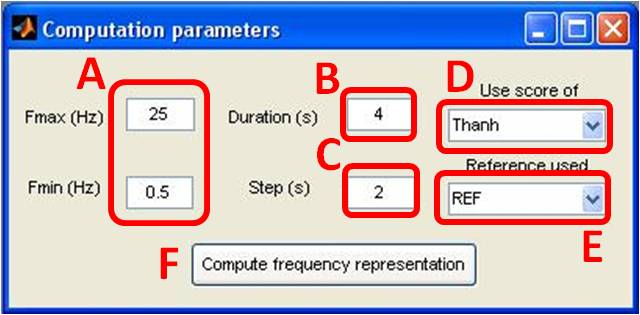
\includegraphics[width=8cm]{images/FIG6_spect_cmp.jpg}
	\caption{Spectrogram calculation GUI: A.~band-pass filtering, B.~time window, C. time step, D.~scorer selection (if available), E.~reference channel, F. launch calculation.
	\label{fig:TB_spect_cmp}}
\end{figure}

If the file was scored using the scoring tool (see section \ref{sec:Sleepscoring}), the sections scored as movement time or marked as artefacts are left out of the spectrogram calculation (power is set to zero). If the file was scored by multiple users, the score to be used is selected via the pull-down menu (Fig.~\ref{fig:TB_spect_cmp}-D).
The artefacted, `movement' or `unscorable' periods are displayed on the spectrogram by blue lines, the width depending on the duration of the arefact, movement/unscorable period. On the frequency band display, the display is just blank at those periods.

The last parameter is the reference taken for the computations (Fig.~\ref{fig:TB_spect_cmp}-E). Once all the parameters have been fixed the user may click on the `Compute spectrogram' button (Fig.~\ref{fig:TB_spect_cmp}-F). When the computation is complete, a ``{\tt .frq}'' file containing the spectrogram is available, and the {\tt file\_array} information (as well as the calculation parameters) are stored in the {\tt D.CRC.pwrspect} substructure.

\subsubsection{Displaying the spectrogram or power spectrum of an M/EEG data file}
%--------------------------------------------------------
\label{sec:spect_dis}
This tool is designed to display the spectrogram computed by the `Compute spectrogram of one EEG file' (cfr. section \ref{sec:spect_cmp}). Two display modes are available (Fig.~\ref{fig:TB_disfrq1}-A): ``Spectrogram'' and ``Frequency band''. ``Spectrogram'' is a time-frequency representation of one channels, dark blue representing low power and bright-red, higher power. A pull-down menu, Fig.~\ref{fig:TB_disfrq1}-B, is used to select the channel to display.

\begin{figure}[ht]
	\centering
		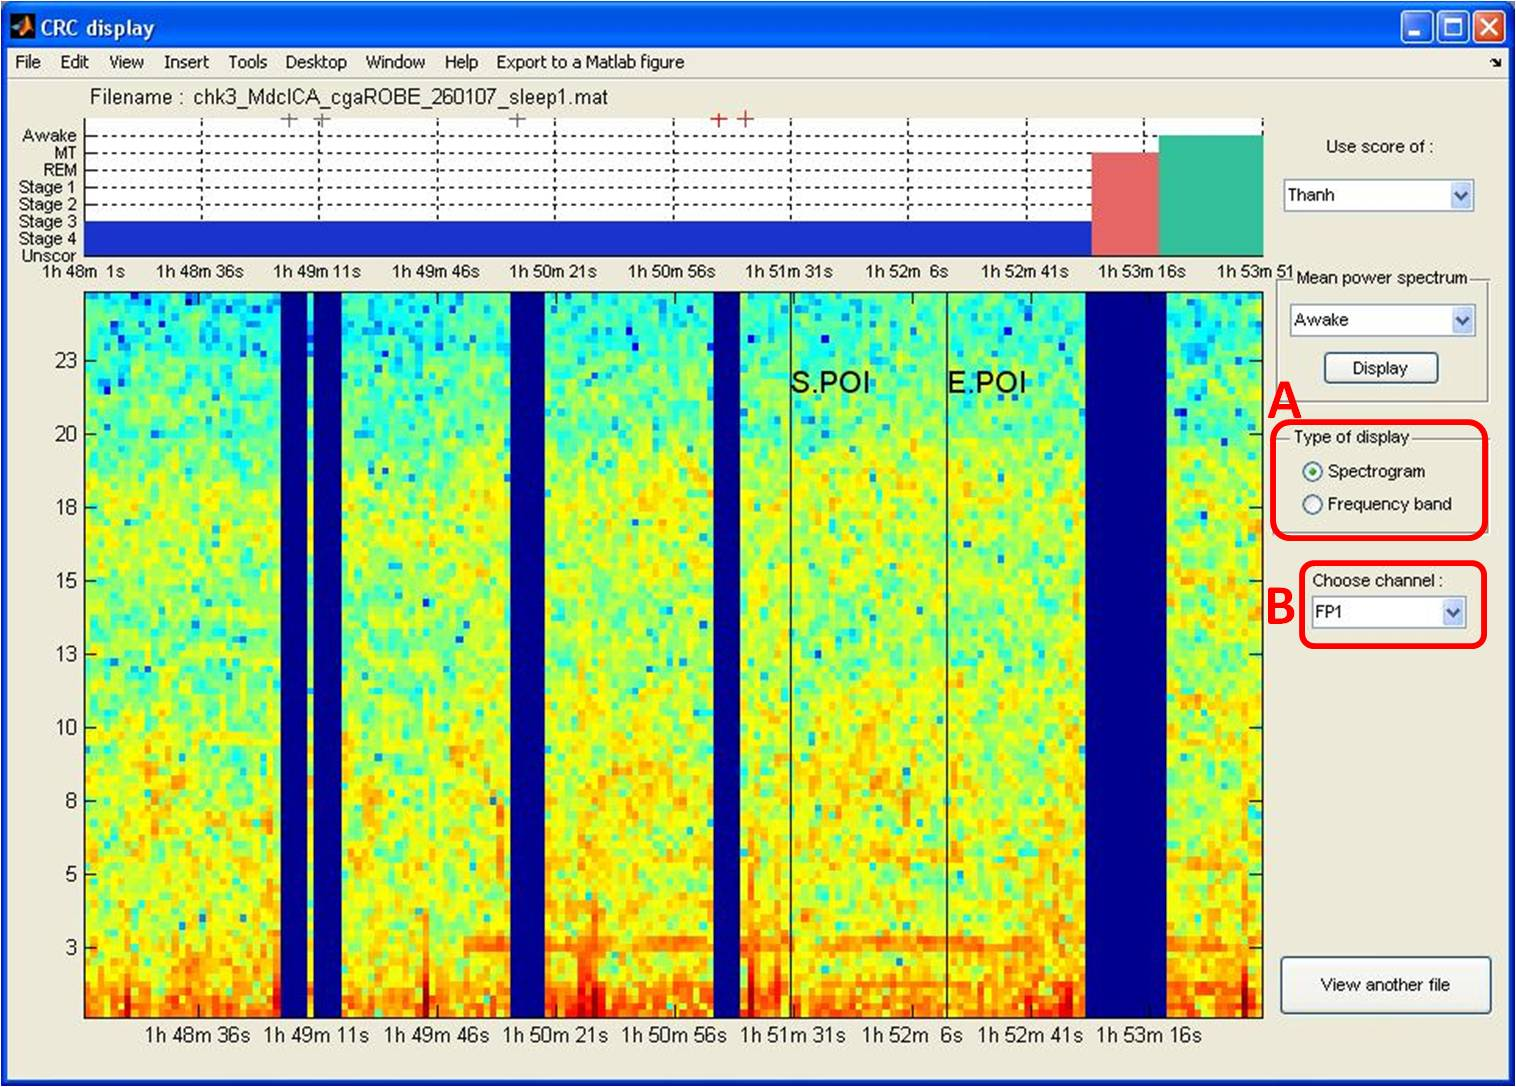
\includegraphics[width=15cm,height=9cm]{images/FIG7_disfreq_spectro.jpg}
	\caption{Main display of spectrogram GUI, ``spectrogram display'': A.~display mode toggle, B.~channel selection.
	\label{fig:TB_disfrq1}}
\end{figure}

In the ``Frequency band'' display mode, the evolution of the power in a specified frequency band (Fig.~\ref{fig:TB_disfrq2}-D) is displayed for one or two channels (channels are picked using 2 pull-down menus, Fig.~\ref{fig:TB_disfrq2}-A). In this display mode, three scaling modes are available (Fig.~\ref{fig:TB_disfrq2}-B): ``Absolute value''; ``Relative value'', i.e. how much power is dissipated at time $t$ in the considered band divided by the whole power at time $t$; and the ``Mongrain view'' (usually used by sleep specialist), it shows the power dissipated at time $t$ in the selected frequency band divided by the mean power in deep sleep stage during the night. Once the scaling mode chosen, the scale itself can be fixed (Fig.~\ref{fig:TB_disfrq2}-C).
\begin{figure}[ht]
	\centering
		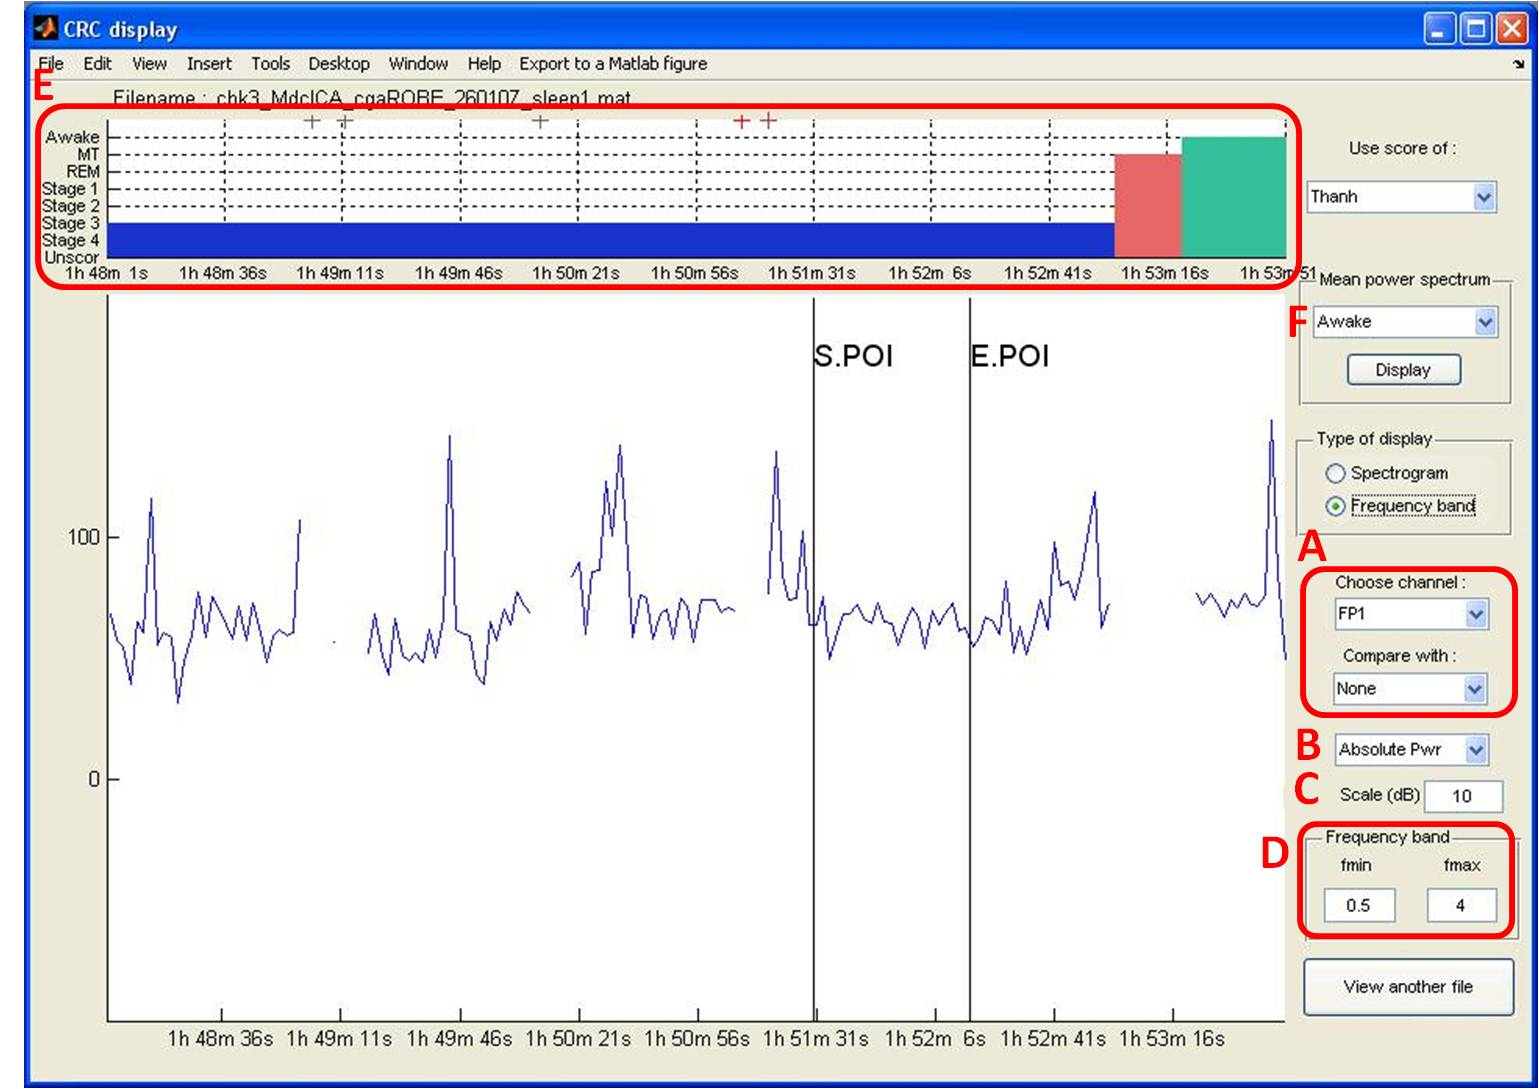
\includegraphics[width=15cm,height=9cm]{images/FIG8_disfreq_fband.jpg}
	\caption{Main display of spectrogram GUI, ``frequency band display'': A.~channel(s) selection, B.~scaling type, C.~scale for display.
	\label{fig:TB_disfrq2}}
\end{figure}

Right clicking on the main plot (either the spectrogram or the frequency band display) lets you define `Periods of Interests' (POI), which will be saved in a new {\tt freq\_POI} field in the data structure, as well as in a text file, along the data set. Periods of Interest are defined in the same way as artefacts in the scoring option: the user defines a start and an end points, which relative times are saved in the data set in seconds. The absolute (if available) or relative times in the hh-mm-ss format of all POIs can be displayed in a new figure using the `POI info' option of the right-click menu. POIs can be deleted by right-clicking on the vertical lines defining either their start or end points.

If the file was previously scored (see section \ref{sec:Sleepscoring}), the hypnogram is also displayed (Fig.~\ref{fig:TB_disfrq2}-E). The user may choose which score to use, and compute the mean power spectrum during a specific sleep stage (Fig.~\ref{fig:TB_disfrq2}-F, results are shown in Fig.~\ref{fig:TB_disfrq3}).
%The `View another file' button allows the user to select another file (Fig.~\ref{fig:TB_disfrq2}-H).
\begin{figure}[ht]
	\centering
		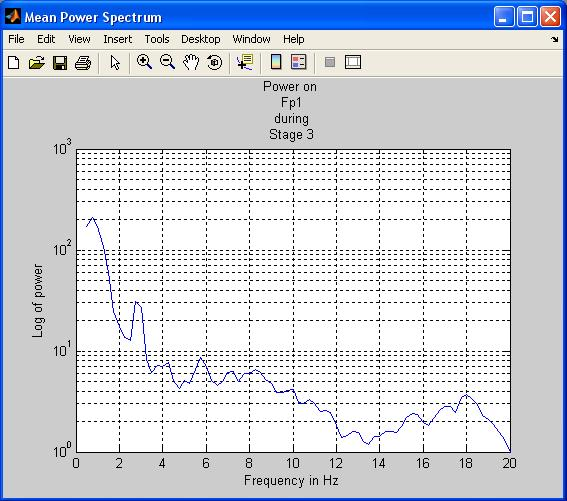
\includegraphics[width=8cm,height=6cm]{images/FIG9_disfreq_pwrstage.jpg}
	\caption{Mean power spectrum during a specific sleep stage (stage 2) for one channel (Oz here).
	\label{fig:TB_disfrq3}}
\end{figure}


\subsection{EEG-MRI artefact rejection tools}
%============================================
\label{sec:eeg_fmri}
In this section we describe the fMRI artefact rejection tools. When EEG is recorded in a MR~scanner during image acquisition (typically fMRI), two types of artefacts are induced on top of the neural EEG signal:
\bi
\item The Gradient Artefact (GA) is induced by the gradient switching of the imaging sequence of the MR scanner\cite{Allen2000}. Note that this several order of amplitude larger than the genuine EEG signal.
\item The Pulse Artefact (PA) is due to the interaction between the {\it static} field of the MR scanner and the heartbeats\cite{Debener2008}. Note that this artefact is thus present even if no fMRI data are acquired.
\ei
One should always suppress the gradient artefact before the pulse artefact.

\subsubsection{Gradient artefact rejection}
%------------------------------------------
\label{sec:gar}
This tool allows the user to remove the Gradient Artefact (GA) resulting from the gradient switching of the MR acquisition sequence. The removal method is based on the ``Average Artefact Subtraction'' (AAS) method developed by Allen et al.\cite{Allen2000}.
AAS estimates the shape of the GA over a TR (the time to acquire a fMRI volume) by averaging the signal over several (typically at least 10) contiguous MR volume acquisitions. This ``averaged artefact'' is estimated for each TR and subtracted from the recorded EEG signal. The efficiency of the AAS approach relies on the stationarity of the GA picked in the EEG signal. This stationarity can be enforced by synchronizing the clocks of the EEG amplifier(s) with that of the MR scanner. This is a crucial point and any user applying this algorithm on data acquired without clock synchronization may (and most certainly will) have improper GA rejection.

This tool is quite simple to use: just select the file(s) you want to correct for gradient artefact. For each file selected, a ``wait bar'' shows you the evolution of the correction and a new data file is (slowly) generated. After corrections your corrected files have the same name as the original ones prefixed with {\tt cga\_} and are available for further processing.
The parameters of the gradient rejection are located in the {\tt crc\_defaults.m} file which you should edit in order to make the program compatible with your specific MR sequence specification and amplifier setup.

There are 2 options to detect the beginning of each scan:
\bi
\item if you record markers coming directly from the scanners to indicate the beginning of each volume (or slice) acquisition, then set the variable {\tt crc\_defaults.gar.UseScanMrk} to 1.  You then have to specify the type of marker you are using in {\tt crc\_defaults.gar.ScanMrk1} (for example {\tt crc\_defaults.gar.ScanMrk1 = 128}\footnote{A secondary marker type can be specified in the field {\tt crc\_defaults.gar.ScanMrk2}.}). If you use slice markers, i.e. one trigger from the scanner every slice, rather than volume marker, you have to set the {\tt crc\_defaults.gar.MrkStep} as the number of slices composing a volume.
\item If you do not record the triggers coming from the scanner (slice or volume) to define the beginning of each volume, set the variable {\tt crc\_defaults.gar.UseScanMrk} to 0. You then have to specify the exact TR of your sequence in seconds ({\tt crc\_defaults.gar.TR} field). You may  automatically detect the beginning and end of the scanning episode in the EEG file using an automatic check \linebreak(field {\tt crc\_defaults.gar.Autochk~=~1}). You can also manually specify the beginning and end of the scanning sequence ({\tt crc\_defaults.gar.beg} and {\tt crc\_defaults.gar.nd}).
\ei

The sampling frequency of the original file (typically 5kHz) is usually higher than necessary for further processing, you can thus specify the sampling frequencey of the output file in \linebreak{\tt crc\_defaults.gar.ouput\_fs} (500Hz by default). The other parameters specify the prefix added to the filename for the corrected file ({\tt crc\_defaults.gar.prefix}), the number of scan on which the average is performed for artefact rejection ({\tt crc\_defaults.gar.Nsc\_aver}) and the number of scans skipped at the beginning of the scanning sequence \linebreak({\tt crc\_defaults.gar.Nsc\_skipped\_be}). Note that the corrected data saved will start at the beginning of the 1st corrected TR, i.e. any pre-scan data are omited. If you're interested in the signal prior that point, then you should extract it (see section \ref{sec:chunking}) from the uncorrected file and possibly append it afterwards (see section \ref{sec:appending}).

\subsubsection{Pulse artefact rejection}
%------------------------------------------
\label{sec:par}
This tool allows the user to reject the ``Pulse Artefact'' (PA) in the EEG recordings. This artefact is induced by the heartbeats of the subject lying in the static field of the MR scanner and is thus present even if no MR data are acquired.

When the tool is launched, the user has to choose which channels will be corrected. Usually EMG or ECG channels are not selected for correction. This step is {\it {\bf crucial} for ICA-based methods}. ICA-based methods are multi-channel methods, i.e. the signal from all the channels are considered together, therefore, if inappropriate (ECG/EMG-like) channels are selected, some EMG information might contaminate EEG data after an ICA-based correction. So you should also ensure that any bad channel(s) are left out from the pulse artefact correction process as they could confuse the ICA-based methods.

Once you have selected the channels to correct for each file, you choose the ECG peak detection method. At the moment the only available method is the one developed by R. K. Niazy and referred to as ``the FMRIB plug-in for EEGLAB'', provided by the University of Oxford Centre for Functional MRI of the Brain (FMRIB) \cite{FMRIBplugin}. We found it very robust even on relatively noisy ECG channels.

After this step, you can choose the type of pulse artefact rejection method you will use. There are five of them: ``PCA'' (FMRIB plug-in), ``Gaussian mean'' (AAS from FMRIB plug-in) \cite{Niazy2005,Iannetti2005a}, ``constrained ICA (automatic)'', ``constrained ICA (manual)'' \cite{Leclercq2009} and ``AAS \& PCA combined'' (based on the FMRIB plug-in)\footnote{a ``multi ICA'' approach \cite{Phillips2006} is also available but not throught the GUI as it takes far too much time to calculate and has not been extensively validated}. The last step lets you choose which channel number is the ECG. If you leave 0, the algorithm will automatically detect~it.

\paragraph{Constrained-ICA method.}
%..........................
Be aware that long episodes with movement artefacts can compromise cICA correction. Indeed cICA works on one time-window (90 seconds by default) at a time and episodes showing ``movement activity'' are not used for the correction estimate (see parameter {\tt crc\_defaults.par.bcgrem.scSNR} here under). So if there is proportionally too much movement during a time-window, not enough ``good'' signal will be available and cICA will not be able to properly decompose the recorded signal and reject the pulse artefact. If you see messages in \matlab command window such as 
\begin{alltt}
Rejecting more than 50\% of time bins from current time window!\\
Warning: Algorithm fails to correct the EEG recordings, probably due to'
too much artefacts.        
\end{alltt}
You should worry about your data: either the gradient artefact rejection did not work so well and your data are still too noisy, or there are some `bad' channels and you should exclude them from the cICA corrections.

Since a seperate cICA correction matrix is estimated and saved for every 90 second time window, it is possible to replace `bad' ones by a better one. The selection of the optimal cICA correction matrix can be automatic (option ``constrained ICA (automatic)'') or manual (option ``constrained ICA (manual)''):
\bi
\item With the automtaic approach a `mutual information'\cite{Peng2005} criteria is used to decide which cICA correction matrix to use: Let's define 2 mutual information measures MI$_1$ and MI$_2$ like this: MI$_1$ = MI(original data, AAS artefact template) and MI$_2$ = MI(corrected data, AAS artefact template). Then the cICA correction matrix leading to the smallest ratio MI$_2$/MI$_1$ is deemed optimal. The MI measures are estimated from random samples of data in the data set, as specified in {\tt crc\_defaults.par.useinitseg}, {\tt .additioseg} and {\tt .length}. Then the corrected data are saved on disk as a new data set. 
\item With the manual approach, no corrected data are saved on disk and the user must decide which correction matrix(-ces) to employ. This selection is performed via the usual display function (see section \ref{sec:dis_main}) and the user can directly visualize the corrected signal obtained by any saved cICA correction matrix. Once the cICA correction matrix is selected, the corrected data are generated and saved on disk in a new data file.
\ei

\paragraph{AAS, PCA and other methods.}
%..........................
We would advise users with 30~channels or more to choose a ``constrained ICA'' (cICA) method. cICA was shown to be more efficient than AAS and PCA at rejecting the PA and to better preserve the spectrum of the ``true'' EEG signal \cite{Leclercq2009}. This is particularly important when analyzing the time course of spontaneous activity (such as in sleep studies). 

With fewer channels ($<$30) or lots of movement activity, single-channel methods are better suited. ``Gaussian mean method'' (AAS)is often preferable but PCA can also do a good job. 
The ``AAS \& PCA combined'' method is experimental and has not been rigorously tested. During the preparation of \cite{Leclercq2009}, we noticed that AAS was more efficient for the lower part of the data spectrum and PCA for the higher part\footnote{In particular, slow waves were sometimes removed by the PCA methods}. ``AAS \& PCA combined'' thus uses a combination of AAS and PCA: AAS is applied on the low-pass filtered ($<$4Hz) signal and PCA on the high-pass filtered ($>$4Hz) signal, then the 2 corrected parts are recombined afterwards.

\paragraph{Specific options.}
%..........................
Users are in effect advised to test test correction methods and find out the ``best'' one for their own data. 
In {\tt crc\_defaults.par.bcgrem}, you can change some parameters linked to the PA rejection, but most of these concern the constrained ICA method such as
\begin{description}
\item[\tt .size] the window size (in seconds) on which cICA is performed;
\item[\tt .step] the step between the beginning of two windows;
\item[\tt .scSNR] the number of standard deviation signal must deviate from to be considered as ``noise'' or ``movement'', i.e. to be exluded from the cICA estimation;
\item[\tt .Refnames] the channels representative of the shape of the pulse artefact;
\item[\tt .NitKmeans] the number of iteration of the K-means step.
\end{description}

\subsection{Sleep specific tools}
%================================
\label{sec:Sleeptools}

These tools and GUI's were specifically developed for sleep data analysis, like the manual scoring of sleep M/EEG (section \ref{sec:Sleepscoring}). The power spectrum of scored data can be estimated and displayed. Finally some summary statistics, about sleeping time, sleep stage duration, etc., can also be calculated afterwards. The spectral power through some sleep stages can also be estimated (section \ref{sec:SleepSpectPwr}).

You can also automatically detect some sleep patterns in your file. This version of \fasst deals with `Slow Waves' (section \ref{sec:SWdetection}) and `Sleep Spindles' (section \ref{sec:SPdetection})\footnote{this latter part of the code is in beta version.}.

\subsubsection{Manual sleep scoring}
%------------------------------------------
\label{sec:Sleepscoring}
Once the user has selected the file to score, the selection channel interface appears (same interface as in section \ref{sec:dis_main}). Once you have selected your favourite channels, hit the `Score' button.

The main display then appears, with all scoring related tools enabled. In particular, a `Scoring' pulldown menu is now visible on the top left of the window. With this menu, you are able to choose the scorer or define another scorer, compare scores, import scores or display grids (vertical every second or horizontal at half of the main scale).
Since this is a scoring tool the size of the displayed time-window is fixed and cannot be changed once it is chosen. 


\begin{figure}[ht]
	\centering
		\includegraphics[width=15cm,height=9cm]{images/FIG11_dis_score.jpg}
	\caption{Sleep scoring GUI, with the hypnogram display on top of the the EEG signal.
	\label{fig:TB_dis_score}}
\end{figure}

If the file is scored for the first time, the program asks a username and a window size. The same file may be scored by different users. To introduce a new scorer, the user has to select ``New scorer'' at the bottom of the scorers option of the `Scoring' menu.

The keypad is used to assign a score to the current window. Each number corresponds to a specific stage\footnote{The labels can be modified in the default file but NOT their number, which is hard coded in some routines.}. By default these are set as: ``Wakefulness'' (0), ``Sleep stage 1-4'' (1-4 respectively), ``REM sleep'' (5), ``Movement Time'' (6), and ``Unscorable'' (7). Each time a score is assigned to the current window, the display moves on to the next time-window. The letters ``b'' and ``f'' can be used to move backward and forward by one time window without assigning any score to the current window. During scoring a hypnogram is automatically constructed and a tick mark shows the current position in the signal. Note that to score a window the main display window has to be selected (i.e. clicked in).

The right-click menu allows the user to add 4 types of events: 
\bi
\item ``artefact \& arousal'', which will be considered as artefact for power spectrum computation, cfr. section \ref{sec:spect_cmp}. Artefacts can be defined in two ways: either as `unspecified' artefacts or as `specified' artefacts. This last option allows to choose a label for the manually defined artefacts, amongst common categories of artefacts (i.e. blink, eye movement, movement). When selecting an unspecified artefact, the label associated to that artefact will be left empty. It is therefore possible to define specified and unspecified artefacts in the same score\footnote{Labels can then be found in the 8th row of the score field created in the data set.}. When defining an artefact (or arousal resp.), the background color of the plot will be changed from white to light blue (light red resp.) to avoid opening an artefact (arousal resp.) without closing it.
\item ``event of interest''. This generic event can be used in different ways depending the interest of the user: for example to manually mark spindles, epileptic discharge,...
\item ``FPL marker'', i.e. ``closing door \& light'' marker (in French ``Fermer Porte \& Lumi\`ere''), to indicate the beginning of the night of recording.
\item `OPL marker'', i.e. ``opening door \& light'' marker (in French ``Ouvrir Porte \& Lumi\`ere''), to indicate the end of the night of recording.
\ei
The latter two, FPL and OPL markers are important to compute sleep statistics.
Artefacts, arousals and events of interest are marked as crosses (respectively grey, red and dark red crosses) on the hypnogram to allow a global visualisation of them along the night.


\subsubsection{Spectral power calculation and statistics}
%------------------------------------------
\label{sec:SleepSpectPwr}
The last item of the right-click pulldown menu is the compute power spectrum tool, same as in section \ref{sec:dis_main}.
These tool are exactly the same as those described in sections \ref{sec:spect_cmp} and \ref{sec:spect_dis}. If the file was scored using the sleep scoring function, the sections scored as movement time or marked as artefacts are left out of the spectrogram calculation (power is set to zero). If the file was scored by multiple scorers, the user has to decide which score to use (Fig.~\ref{fig:TB_spect_cmp}-D).

The hypnogram is also displayed (Fig.~\ref{fig:TB_disfrq2}-E) alongside the spectrogram display. The user may choose which score to use, and compute the mean power spectrum during a specific sleep stage (Fig.~\ref{fig:TB_disfrq2}, results are shown in Fig.~\ref{fig:TB_disfrq3}).

Finally the `Compute Statistics' button is accessible via the `Scoring' pull-down menu: the proportion of the different sleep stages, of the movement time and of the wakefulness stage, the latency of REM sleep, etc. are then displayed (Fig.~\ref{fig:TB_dis_score2}).

\begin{figure}[ht]
	\centering
		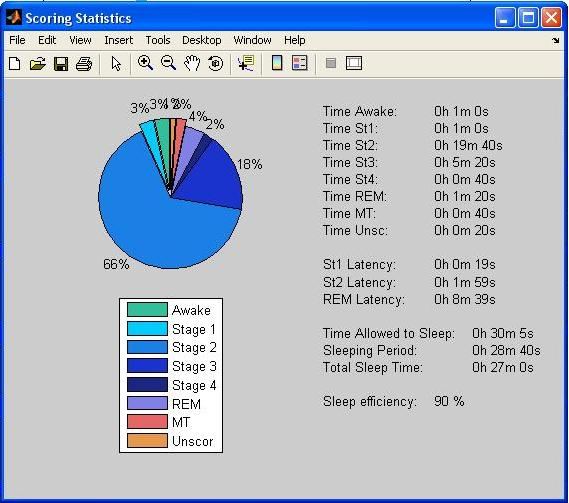
\includegraphics[width=10cm]{images/FIG12_score_stats.jpg}
	\caption{Sleep statistics results.
	\label{fig:TB_dis_score2}}
\end{figure}


\subsection{Automatic wave detection tools}
%==========================================
\label{sec:WaveDetect}

Automatically extrating features from continuous EEG recording is a complicated task mainly because of the poor signal-to-noise ratio and the variability (within and between subjects) of the ``waves'' to detect. We focused on two types of spontaneous sleep waves, namely ``slow waves'' and ``spindles''. The methods are described in the next two sections. Still, when using these tools, keep in mind that wave detection is not ``bullet proof'' and paramter may need to be tweaked to achieve the best results on your data.

\subsubsection{Slow Wave detection}
%------------------------------
\label{sec:SWdetection}

This tool aims at detecting Slow Waves (SWs) in a EEG recording. 
SWs detection is performed on the averaged ROI signals (i.e. over 4 averaged signals in the case of automatic selection of ROI, see here under). The detection was designed in a spatio-temporal way following Massimini's criteria \cite{Massimini2004} but were adapted according to our observations on different data sets (Fig.~\ref{fig:SWS_crit}):
\begin{enumerate}
\item A negative zero crossing (down-zero crossing) and a subsequent positive zero crossing (up-zero crossing) separated by 0.25-1.25sec,
\item A negative peak between the two zero crossings with voltage $<$ -80$\mu$V,
\item A negative-to-positive peak-to-peak amplitude $>$ 140$\mu$V,
\item A positive slope $>$ 90\% of the maximum slope, 
\item A positive zero crossing and a subsequent positive peak separated by maximum 2 sec.
\end{enumerate}
\begin{figure}[ht]
	\centering
		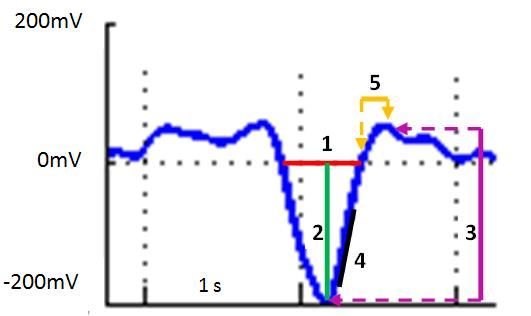
\includegraphics[width=7cm]{images/FIG16_SWS_criteria.jpg}
	\caption{SW detection criteria: (1)	A negative zero crossing (down-zero crossing) and a subsequent positive zero crossing (up-zero crossing) separated by 0.25-1.25sec, (2) A negative peak between the two zero crossings with voltage $<$ -80$\mu$V, (3)	A negative-to-positive peak-to-peak amplitude $>$ 140$\mu$V, (4)	A positive slope $>$ 90\% of the maximum slope, (5)	A positive zero crossing and a subsequent positive peak separated by maximum 2 sec.
	\label{fig:SWS_crit}}
\end{figure}

Each detected SW is used to build a ``SW trajectory" over the scalp, using all the channels. Channels presenting a SW are detected and a ``delay value'' is estimated for each of them, based on the difference between the negative peak time at this electrode and the negative peak time at the first electrode detecting the specific SW. A code is also attributed to each wave in function of its type (delta or SW). No user participation is required.

The detection procedure relies on the following steps:
\begin{enumerate}
\item Extraction of the data within a time window of interest in the provided file,
\item Filtering between 0.2 and 4 Hz of the extracted data,
\item Creation of Regions of Interest (ROI),
\item preliminary SWs detection on the signals averaged over ROI,
\item Detection of each SW on all the channels.
\end{enumerate}
Once the SWs are detected, the trajectory of the peak negativity  over the scalp surface is also extracted using the information from all channels (SW detection and channel location). Finally the SWs are displayed.

The characteristics of the detected waves are saved in a new field {\tt D.CRC.SW} of the original data structures\footnote{For more information on this field content, type  {\tt help crc\_SWS\_detect} at the Matlab prompt.}. Their most important characteristics are also saved in the field {\tt D.events} to allow an easy epoching of the waves. This  new field {\tt D.CRC.SW} is also saved in the chunked and SW files if the option in `Analyse' was not `all file'. In that case, the time characteristics of the waves will be relative to the start of the input file in its SW field while they will be relative to the start of the chunked or SW file in theirs. This allows using either the input file or the chunked/SW file for SW analysis, according to what suits your needs best.

After clicking on `SWS detection' in the main \fasst window, a GUI appears and lets you specify the parameters of the detection procedure (Fig.~\ref{fig:sws_detect_gui}).
This interface is divided into four main parts: the EEG file selection (on top), analysis parameters (left), review parameters (middle right) and parameters specific to joint EEG-fMRI data (bottom right).
\begin{figure}[ht]
	\centering
		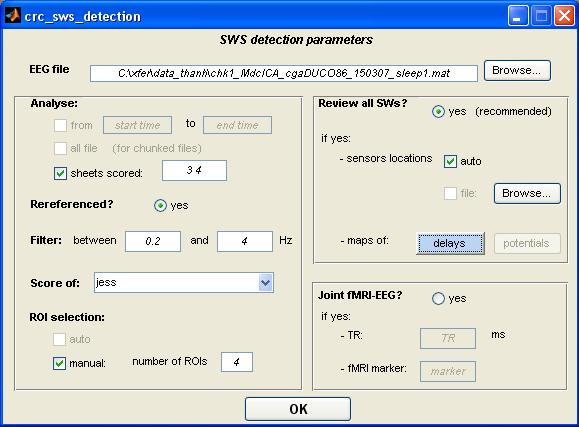
\includegraphics[height=7cm]{images/FIG14_SWS_gui.JPG}
	\caption{User interface allowing for the specification of the different steps parameters
	\label{fig:sws_detect_gui}}
\end{figure}

\paragraph{Analysis parameters.} These are the parameters of the detection procedure (time window, filtering, etc.), the thresholds used for the detection itself are defined in the {\tt crc\_defaults.m} file.  
\bi
\item {\bf Time window selection.} This step allows extracting data of interest within the provided file. Three options are available:
\begin{description}
\item[\tt from ... to ....] chunks the file according to the user specified times. If the file contains time information (typically if it was imported using \fasst), the `start time' and `end time' fields should be specified in real-world time (for example, [23~45~02] for `23h~45m~2s'). Otherwise, they should be considered as relative times, 0h 0m 0s being the start of the input file. In all cases, the correct format for those entries is: hh-mm-ss.
\item[\tt all file] for already chunked files or small files containing only Slow Wave Sleep (SWS) stages. The SWs detection is performed directly on this file, without the creation of any other file.
\item[\tt sheets scored] builds a new file from the concatenation of all sheets scored `scores' (specified by spaced numbers, e.g. 3 4). This new file is stored on the drive under the name {\tt SW\_filename}. This option is particularly useful if there is no specific moment of interest in the file: if the input file is a whole night recording and by specifying the scores as~3 and~4, the SWs detection will be performed on all SWS stages.
\end{description}
Note that, in all cases, periods marked as artefacted (artefacts or arousals) or as movement time or unscorable will be skipped from the analysis.

\item {\bf Re-reference parameters.}
The algorithm checks for a re-referencing operation in the field {\tt D.history} (modified after each SPM8 processing). If it does not find such an operation, the user is asked if he wants to continue or not. Please, apply your montage before any processing of the data.
%\ei

\item {\bf Filter parameters.}
If the file wasn't filtered in the frequency band of interest, the procedure will band-pass filter the data (by default, 0.2-4Hz) by applying first a 0.2Hz highpass filter and then a lowpass filter with cutoff frequency at 4Hz to ensure stability. No files are created from this operation. If such filtered files are useful for you, you should preferably first filter the data in SPM8 and specify the newly created file as input. The filters used are the same as those of SPM8 (Butterworth type)
\footnote{For data sets with a relatively high sampling rate (up to 500 Hz), the user should enlarge the frequency bands to ensure the stability of the filters. Another parameter which can be modified is the order of the filter. For the Butterworth filters used in this toolbox, the default value is 4. However, decreasing this order leads to an increased stability. If the user wants to keep the defaults settings, he should downsample his file.}.

\item {\bf Scorer Pull down menu.} To choose the scorer's score to use.

\item {\bf ROI selection parameters.}
To decrease the computational load, SWs detection is first performed on averaged signals over (typically) 4 ROIs: frontal, central left, central right and parietal. Two options are available for the channel selection: 
\begin{description}
\item[\tt automatic] Channels in a radius (below about 15\% of scalp radius) around the 2D normalized flattened positions of respectively Fz, C3, C4 and Pz channels in the extended 10-20 system\footnote{If the file was previously prepared within SPM8, the algorithm will select the coordinates saved in the data file. Otherwise, theoretical positions will be used ({\tt crc\_electodes.mat}).}; 
\item[\tt manual] You need to specify the number of ROI desired and their names. The ROI specification is then performed for each ROI in order. This manual selection is based on the channel selection GUI (see section \ref{sec:dis_main} and Fig.~\ref{fig:SWS_roisel}). Already hand-built ROI selections can be loaded and saved via this GUI.
\end{description}

In case your file has not been previously prepared in SPM8 and for an optimal electrode selection (manual or automatic), please edit the {\tt crc\_electrodes.mat} via the matlab script {\tt crc\_electrodes.m} if you have other electrodes systems than BrainProducts or EGI systems. 
\begin{figure}[ht]
	\centering
		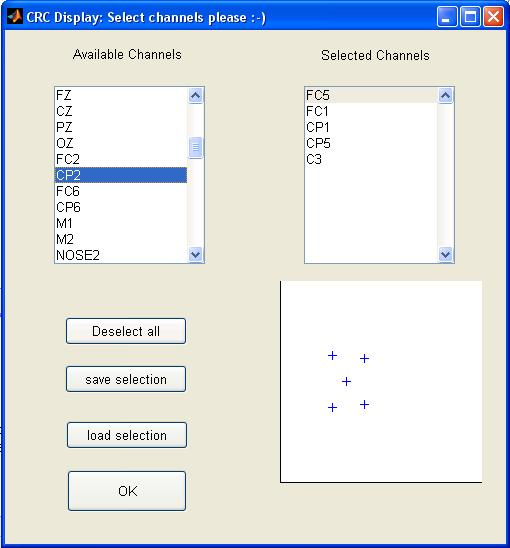
\includegraphics[height=7cm]{images/FIG15_SWS_ROI_sel.JPG}
	\caption{User interface allowing for a manual selection of ROI channels
	\label{fig:SWS_roisel}}
\end{figure}
\ei

\paragraph{Display parameters.}
When answering `yes' to the `Review all SWs?' question, 
the main display appears after the end of the detection. The user has to choose the channels to display and select either `SW' or `delta' types in the `Events' panel to review the detected waves. In case no other events were present in the data set, `All' can also be selected and will show both types of slow waves.
If the 'delay map' was selected previous to the wave detection, a delay map will appear in the bottom right corner of the display in an inverted hot colormap (Fig.~\ref{fig:SWS_dis}).

To compute the interpolated values, the algorithm needs the 3D position of the electrodes. This is specified by ticking the `file' option under the `sensors locations' parameters. However an `auto' option is available, which will compute a 2D interpolation of the signal based on the 2D sensors positions. 
Once again, the algorithm will check if the coordinates were assigned to the channels ({\tt spm\_eeg\_prepare}) or not. In the latter case, to obtain a good interpolation, please edit the {\tt crc\_electrodes.mat} via the matlab script {\tt crc\_electrodes.m} or SPM8 GUI, if you have other electrodes systems than BrainProducts or EGI systems. Please note that, for the moment, the `auto' option is only available if you display maps of delays.

\begin{figure}[ht]
	\centering
		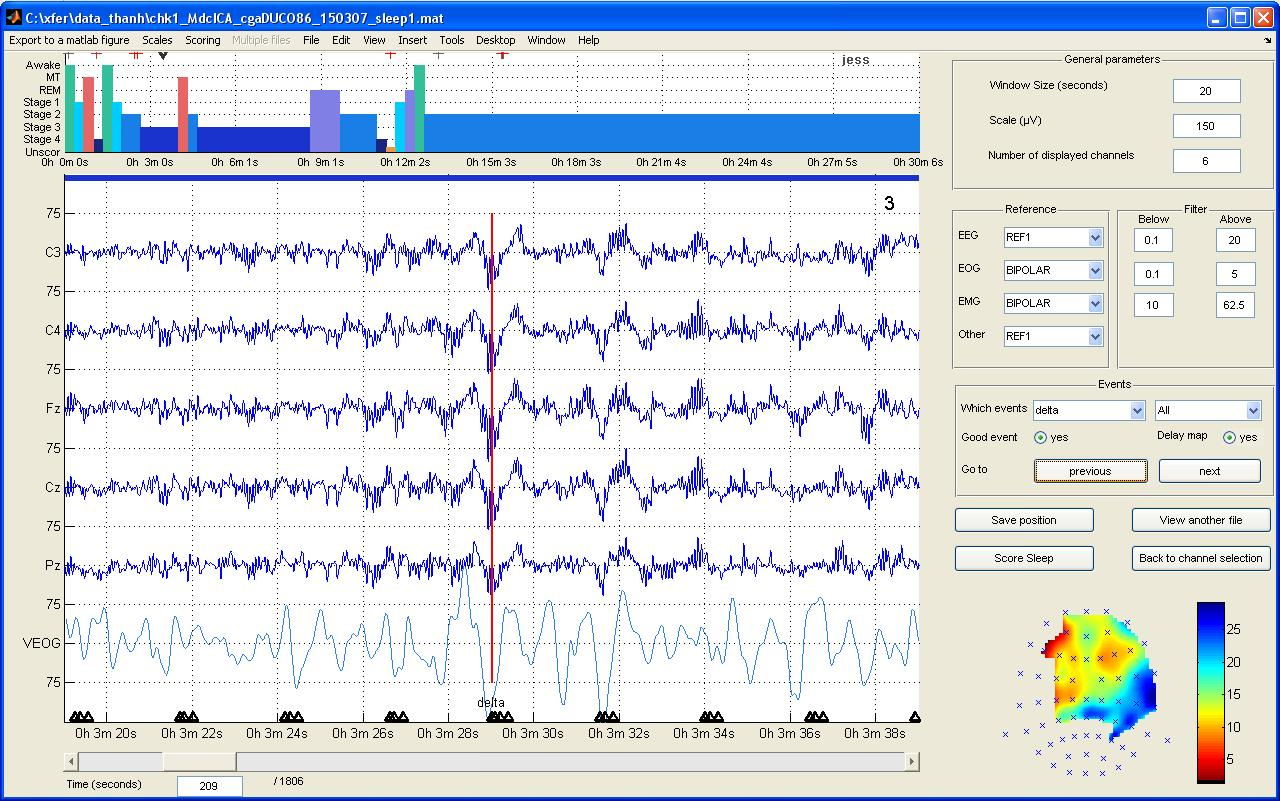
\includegraphics[width=15cm]{images/FIG17_dis_SW.jpg}
	\caption{Sleep scoring display with a colour-coded delay map (scale is in ms) in lower right corner.
	\label{fig:SWS_dis}}
\end{figure}

\paragraph{Joint EEG-fMRI acquisitions.}
Due to the growing use of combined EEG-fMRI techniques, the toolbox can compute the main SW characteristic in units of TR, if the EEG recordings has an identifiable event (marked with `marker') indicating the start of the MRI recording. Therefore, by specifying the TR and this marker, the value of the negative peak maximum power can be computed in terms of TR. This information is stored in the SW structure contained in the {\tt D.CRC.SW} field under the name {\tt negmax\_TR}. Please note that this computation only takes into account a shift between the start of the EEG recording and the beginning of the scan. If the relationship between the timing of your EEG and fMRI recordings is more complex, use this tool carefully.

Please note that when repeating a SW detection on the same file, any event with a `SW' or `delta' type will be erased to avoid redundancy. The field {\tt goodevents} will also be reset since the number of events was changed.

\subsubsection{Sleep Spindles detection {\itshape\bfseries (BETA version!)}}
%------------------------------
\label{sec:SPdetection}

%\paragraph{Detection principles}
The spindle detection algorithm was derived from the method described by M. M\"{o}lle et al. \cite{Moelle2002}. To match empirical results obtained with different data sets, some of the detection parameters were however adjusted. 

To reduce computational effort, the detection is performed on 3 `reference' channels (i.e. Fz, Cz and Pz) only; these channels are selected according to their scalp position (the channels being closest to the theoretical positions of the 3 channels of reference will be selected). The 2D positions considered for channels are the coordinates saved by the SPM8 preparation step. If this step was not performed, the positions will be retrieved from the {\tt crc\_electrodes.mat}. In this last case, you must ensure that the system used to acquire the data is supported by this file (otherwise, you need to edit then run the file {\tt crc\_electrodes.m}). The algorithm will then check that none of these channels are bad. If this condition is not fulfilled, the detection is interrupted. For the moment, the only way to perform spindle detection with one of the reference channels being `bad' is to change the channels of interest for that particular file in the file {\tt crc\_defaults.m}.

The signal from the reference channels is extracted, discarding all artefacted/arousals, movement or `unscorable' periods, and filtered (user-defined frequency band, Butterworth bandpass filter). According to  \cite{Moelle2002}, only the largest spindles are to be considered and, therefore, thresholds have to be computed. In our implementation, the thresholds are computed as the percentile 95 of the extracted signal of the reference channels scored as sleep stage 2 (and only this stage). Three thresholds are obtained, one for each reference channel. These thresholds are displayed in the workspace, and, as in \cite{Moelle2002}, are usually within 5$\mu$V of each other. % ($\leftarrow$ JESSICA, 3 values within 5 $\mu$V from each other, or their absolute value???)

Example of workspace display: 
\begin{center}
%\begin{quotation}
\begin{verbatim}
	....................................................
	....... Computing RMS and detecting spindles .......
	....................................................
	Threshold of detection for channel Fz : 13.9959
	Threshold of detection for channel Cz : 12.7297
	Threshold of detection for channel Pz : 11.859
\end{verbatim}
%\end{quotation}
\end{center}
A root mean square (RMS) signal is then computed from the previously extracted signals (all user defined stages or time period), using a rectangular window of 0.1 second and a time resolution of 0.05 second. A binary signal is then computed: whenever the RMS signal is larger than the previously computed corresponding threshold, the value is 1, otherwise it is 0 (Fig.~\ref{fig:SP_datarms}). The average of the 3 binary signals is then computed and ceiled (i.e. whenever there was a 1 on one binary signal, there is a one on the ceiled signal). Using this ceiled average, one can detect bursts of activity in the frequency band of interest lasting at least 400ms and separated by at least 1000ms, which are then considered as spindles. This last criteria was added to those of M. M\"{o}lle et al. \cite{Moelle2002}, according to our experimental results, to reduce of false positive detection.
\begin{figure}[ht]
	\centering
		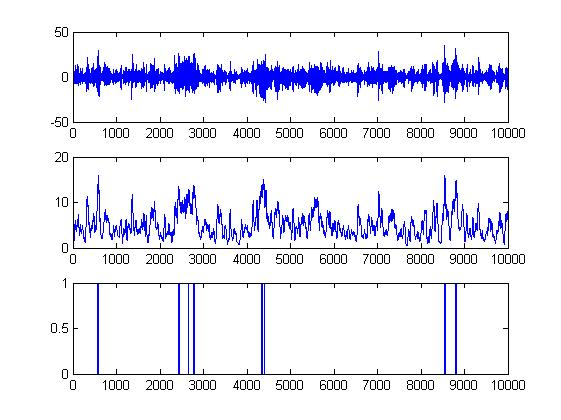
\includegraphics[width=12cm]{images/FIG18_SP_datarms.jpg}
	\caption{Illustration of the spindle detection using the extracted (top plot), RMS (middle plot) and binary (bottom plot) signals on Cz, the threshold being 12.7297$\mu$V as computed previously.
	\label{fig:SP_datarms}}
\end{figure}  

%\paragraph{Detection using \fasst}
After selecting of the `spindles' detection in the wave detection tool, the user has to define the different parameters of the spindles detection (Fig.~\ref{fig:SP_gui}).
\begin{figure}[ht]
	\centering
		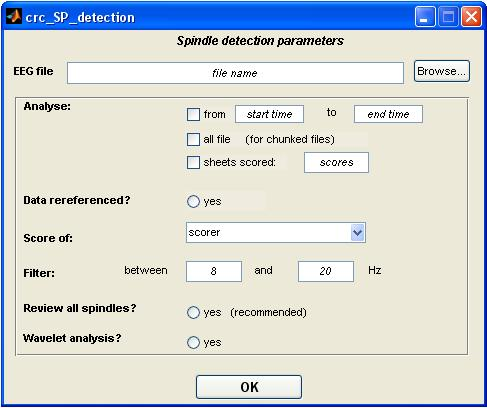
\includegraphics[width=7cm]{images/FIG19_SP_gui.JPG}
	\caption{Graphical user interface allowing to define the parameters of the spindle detection.
	\label{fig:SP_gui}}
\end{figure}

\bi
\item {\bf EEG file.}
To select the input {\tt .mat} file corresponding to the data set to analyze. The name of the file can either be typed in manually or browsed.

\item {\bf Analyze.}
Options similar to those of the SW detection (see previous section).

\item {\bf Data rereferenced?}
To check if the file was already rereferenced.

\item {\bf Score of.}
To choose the scorer. Please note that this step determines the time periods used since artefacts, arousals, movement or unscorable periods will be withdrawn from further analysis.

\item {\bf Filter.}
Choose the filter to apply. Different tests on data sets showed that the 8-20 band was optimal for spindles detection. Therefore, if you want to reduce that band (for example to 12-15 Hz), please note that filter ripples can affect the signal.

\item {\bf Review all spindles?}
Check if you want to review the spindles after detection. This option launches the main display after the detection. After choosing the channels to display (reference channels are preselected), go to the `Events' panel and choose to display `SP' types (`Ant\_SP' or `Post\_SP' if the next option is selected) and `All' values to review the detected spindles (Fig.~\ref{fig:SP_detect}). Please note that some spindles are not visible when Slow Wave activity is displayed simultaneously. Therefore, changing the filters might be useful (one possibility might be to choose the frequency band used to detect the spindles).
\begin{figure}[ht]
	\centering
		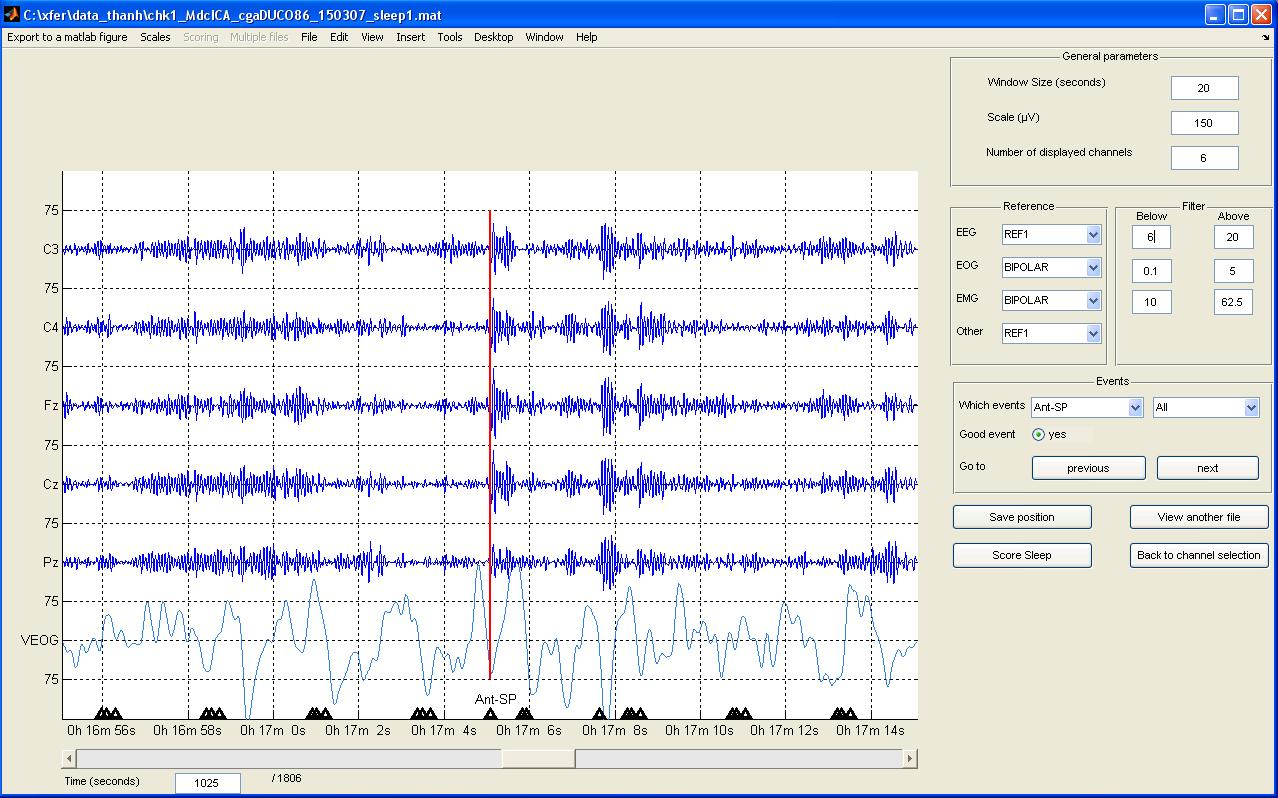
\includegraphics[width=15cm]{images/FIG20_dis_SP_detect.JPG}
	\caption{Review of detected spindles (here anterior spindles) on the reference channels.
	\label{fig:SP_detect}}
\end{figure}

\item {\bf Wavelet analysis?}
This option performs a wavelet analysis of the detected spindles (previously epoched around their starting time). The power spectra on the anterior and posterior channels in the band 11-16Hz are then compared and the spindle is then labeled as `anterior' (Ant-SP) or `posterior' (Post-SP) according to the largest power spectrum. The anterior or posterior character of the channels is computed according to their y-coordinate, the reference being Cz (theoretical 2D coordinates: $[0.5\;0.5]$). Therefore, using theoretical 2D coordinates ({\tt crc\_electrodes}) or preparing the file using SPM8 can lead to slightly different results as different electrodes could be picked as references.
\ei

During detection, different characteristics of the spindles are computed, such as their starting and ending points, their duration, the maximum amplitude and the channel on which it occurred. When the wavelet analysis is selected, the `anterior' or `posterior' character of the spindles is also computed, as well as their frequency. All these parameters are saved in the data set ({\tt D.CRC.spindles}) and spindles are considered as events (to epoch the spindles if needed, codes 777 for `SP', 555 for `Ant-SP' and 666 for `Post-SP'), which can therefore be marked as `good' or `bad' during reviewing.

%%%%%%%%%%%%%%%%%%%%%%%%%%%%%%%%%%%%%%%%%%%%%%%%%%%%%%%%%%%%%%%%%%%%%%%%%%%%%%%
\section{Advanced Users}
\label{sec:advus}
%%%%%%%%%%%%%%%%%%%%%%%%%%%%%%%%%%%%%%%%%%%%%%%%%%%%%%%%%%%%%%%%%%%%%%%%%%%%%%%
The first part of this section describes the fields added by \fasst to the standard SPM8 structure/object (.mat file). These additional fields do NOT interfere with SPM8 machinery, they merely contain extra-information used by \fasst for the time-frequency analysis, sleep scoring and wave detection. The second part is dedicated to the functions not accessible from the main GUI.

\subsection{Addition to the SPM8 structure}
%=============================================
As stated previously \fasst does not modify the main fields of the SPM8 structure, except when events are added, and all additional structures are placed in seperate subfields ({\tt info} and {\tt CRC} at the moment). %The SW detection tool being still a {\it beta} version and prone to changes, the added fields are not explicitly described here.

\subsubsection{The {\tt D.info} field}
%-------------------------------------
When \fasst creates a {\tt .mat} header from a {\tt .vhdr} one (BrainProducts Recording System), the time and the date at the beginning of the recording are stored respectively in the {\tt D.info.hour} and {\tt D.info.date} fields. Note that when these informations are available, the time axis of the different display (scoring, display, frequency representation) is expressed in ``clock time'', otherwise it is expressed in ``relative time'' from the beginning of the recording.

\subsubsection{The {\tt D.CRC} field}
%-------------------------------------
\paragraph{Spectrogram information}
When the spectrogram of a file is computed, several bits of information are added to the structure {\tt C.CRC.spectpwr}:
\bi
\item {\tt .frqname} contains the file name of the spectrogram data;
\item {\tt .frqNsamples} is the number of instantaneous power spectra computed for each channel;
\item {\tt .frqNbins} is the number of frequency bins for the spectrogram;
\item {\tt .frqdata} is the {\tt file\_array} pointing to the spectrogram data, use it as a matrix;
\item {\tt .frqscale} is the scale factor for each channel;
\item {\tt .frqbins} contains {\tt frqNbins} elements which are the centre of the frequency bins in Hz;
\item {\tt .step} is the step (in seconds) between two window used to compute two following power spectra;
\item {\tt .duration} is the length (in seconds) of the windows used to compute the power spectra;
\item {\tt .frq\_POI} contains the time (in seconds) of the user-defined `Periods of Interest'.
\ei

\paragraph{Scoring information}
When a file has been scored at least one time, a cell array {\tt D.CRC.score} of dimension $8\times N$ is added to the structure, where $N$ is the number of scorer(s). Each column contains the details of one score, from row one to seven:
\bi
\item a $1\times R$ vector containing numbers representing the score, where $R$ is the number of scoring windows. ``Stage'' labels  are defined in the {\tt crc\_defaults.m} file. By default they are set as: 0 correspond to ``Wakefulness'', 1-4 to ``Sleep stage 1-4'' respectively, 5 to ``REM sleep'', 6 to ``Movement Time'', and 7 to ``Unscorable'';
\item the name of the scorer;
\item the length of a scoring window (in seconds);
\item two numbers indicating the time when the light was shut off and door was closed (FPL, first number), and when the light was turned on and the door was opened (OPL, second number). These measures are given in seconds relative to the beginning of the file;
\item a $2\times T$ array, where $T$ is the number of artefacts scored. The first column is the beginning of each artefactual episode and the second, the end of it. All the times expressed in seconds relative to the beginning of the file;
\item same as artefacts but for arousals;
\item same as artefacts but for events of interest;
\item a $1\times T$ cell array, containing the label of each artefact. The labels for 'unspecified' artefacts are left empty.
\ei

\paragraph{SW detection information}
Other fields added to the {\tt D.CRC.SW} object for the SW detection:
\bi
\item {\tt .SW}, a $1\times T$ structure array, $T$ being the number of detected waves, containing all the properties of the waves (type {\tt help crc\_sws\_detect} for the specification of these fields);
\item {\tt .origin\_count}, a $N\!el\times 3$ cell array, $N\!el$ being the number of non bad EEG electrodes in the file. This array contains, for each electrode (column 1), the number of waves first detected on that electrode (column 2) and the total number of waves detected on this electrode (column 3).
\ei

\paragraph{Spindle detection information}
Other fields added to the {\tt D.CRC.spindles} object for the SP detection:
\bi
\item {\tt D.spindles} contains different properties of the spindles, each in the $N\!sp\times k$ size, $N\!sp$ being the number of detected spindles and $k$ depending of the subfield. All fields are explicit, except {\tt maxelectrodes}, which contains the electrode on which the spindle has maximum amplitude.
\ei

\paragraph{Other information}
Other fields added to the {\tt D.CRC} structure for display management:
\bi
\item {\tt .lastdisp}, time in seconds saving the position when clicking on the 'save position' button;
\item {\tt .goodevents}, a $1\times N\!ev$ vector of binary elements, $N\!ev$ being the number of events in the file, as in the {\tt D.events} field. 1 represents events marked as good (default) while 0 represents events marked as `bad' via the display.
\ei

\subsection{``Hidden'' functions}
%================================
{\tt crc\_statgen} can only be used on files which were previously sleep-scored and computes statistics such as the percentage of the different sleep stages, the latency of the sleep stages, the efficiency of sleep, the total sleep time, the number of arousal per hour, etc. The function creates a text file,  named {\tt Statgen.txt}, with these values and also return a matrix in the \matlab workspace. The content of this file can be copy-pasted in a cell-formated program such as Excel. If more than one file is selected, then the text file and the matrix will contains as many lines as there are selected files.

%%%%%%%%%%%%%%%%%%%%%%%%%%%%%%%%%%%%%%%%%%%%%%%%%%%%%%%%%%%%%%%%%%%%%%%%%%%%%%%
\section{Acknowledgments}
\label{sec:ackn}
%%%%%%%%%%%%%%%%%%%%%%%%%%%%%%%%%%%%%%%%%%%%%%%%%%%%%%%%%%%%%%%%%%%%%%%%%%%%%%%

This M/EEG toolbox is developed with the financial support of the Fonds de la Recherche Scientifique-FNRS, the Queen Elizabeth fund, and the University of Li\`ege.

The authors would like to thank the CRC staff for their comments and suggestion during the development of \fasst\hspace{-4pt}. A special thank goes to Virginie Sterpenich and Christina Schmidt whose suggestions were very helpful during the design and the very birth of \fasst\hspace{-4pt}, and also to Pierre Maquet who imagined \fasst before we made it real. We are also grateful to all the users at the CRC (especially Luca Matarazzo, Ariane Foret, Laura Mascetti and Thanh Dang Vu) who helped us debug the code by boldly using the alpha version of the toolbox. Thanks also go to the ``foreign labs'' who provided some data sets to test the reading functions and the MR-artefact rejection tools.


\bibliography{FASST_manual}
\end{document}
